%% Copyright 2023 P. S. Eduardo.
%
% This work may be distributed and/or modified under the
% conditions of the LaTeX Project Public License, either version 1.3
% of this license or (at your option) any later version.
% 
% The Current Maintainer of this work is P. S. Eduardo.
%
% This work consists of the file poli.cls.
%% -----------------------------------------------------------------
% Escola Politécnica UFRJ LaTeX Template
% Version: 2302
% Author: Eduardo Paiva dos Santos
% email: eduardopaiva@poli.ufrj.br
% Base: CoppeTeX 2.3
%%------------------------------------------------------------------
\documentclass[grad,pdftex]{poli}
\usepackage[utf8]{inputenc}
\usepackage{amsmath,amssymb}
\usepackage{float}
\usepackage{multirow}
\usepackage{longtable}
\usepackage{tikz}
\usetikzlibrary{shapes,arrows,chains,positioning}
\usepackage{enumitem}
\usepackage{indentfirst}
\usepackage{array}
\usepackage{diagbox}

%\usepackage[alf, bibjustif]{abntex2cite}

\makelosymbols
\makeloabbreviations

% ======== ADDED BY MARIO ======== %
% Reference numbers
\usepackage[numbers]{natbib}

% PlantUml diagrams
\usepackage{svg}

% Code blocks
\usepackage{listings}
\usepackage{color}
\definecolor{d-blue}{HTML}{001080}
\definecolor{blue}{HTML}{0000ff}
\definecolor{gray}{rgb}{0.5,0.5,0.5}
\definecolor{d-red}{HTML}{A31515}
\definecolor{pink}{HTML}{af00db}
\def\beginlstdelim#1#2#3%
{%
    \def\endlstdelim{#2\egroup}%
    \ttfamily#1\bgroup\color{#3}\aftergroup\endlstdelim%
}
\lstset{frame=tbrl,
  showstringspaces=false,
  % columns=flexible,
  basicstyle={\small\ttfamily},
  numbers=left,
  % numberstyle=\tiny\color{gray},
  identifierstyle=\color{d-blue},
  numberstyle=\color{gray},
  keywordstyle=\color{pink},
  emph=[1]{protected, private, public, static, final, extends, implements,
           global, if, else, foreach ,for,
           endforeach, endif, endfor, elseif,
           as, try, catch, require_once},
  emphstyle=[1]\color{pink},
  emph=[2]{use, new},
  emphstyle=[2]\color{blue},
  moredelim = **[is][\beginlstdelim{@>}{(}{pink}]{@>}{(\$)},
  commentstyle=\color{gray},
  stringstyle=\color{d-red},
  breaklines=true,
  breakatwhitespace=true,
  tabsize=4,
  showlines=true
}

% Directory Tree
\usepackage{dirtree}

% Numero em subsubsection
\setcounter{secnumdepth}{3}

% Bar chart
\usepackage{pgfplots}
\usepackage{pgfplotstable}
\pgfplotsset{
    compat=1.9,
    compat/bar nodes=1.8,
}
% ======== ADDED BY MARIO ======== %


\begin{document}
  \title{Architectural Patterns to Support the Development of REST APIs at CERN}
  \foreigntitle{TCC Title}
  \author{Mario}{Günter Simão}
  \advisor{Prof.}{Flávio Luis}{de Mello}{D.Sc.}
  %\coadvisor{Prof.}{Nome}{Sobrenome}{D.Sc.}
  \examiner{Prof.}{Nome Completo}{Ph.D.}
  \examiner{Prof.}{Nome Completo}{D.Sc.}
  %\examiner{Prof.}{Nome Completo}{D.Sc.}
  \department{DEL} %UTTILIZE A SIGLA DO SEU DEPARTAMENTO MODIFICAR OS NOMES DE CURSO, DEPARTAMENTO E OBTENÇÃO DE GRAU (Obs: caso tenha algum equívoco nesses argumentos, necessário modificar o arquivo poli.cls no local que faz a leitura deste argumento)
  \date{6}{2023}
  \keyword{keyword1}
  \keyword{keyword2}
  \keyword{keyword3}
  \keyword{keyword4}
  \maketitle

  \frontmatter
  \dedication{``Uma frase de dedicatória qualquer'' - Autor desconhecido.}


  \chapter*{Acknowledgements}

I would like to express my sincere gratitude to all the individuals who have supported and guided me throughout the journey of completing this undergraduate thesis. Their encouragement and assistance have been invaluable in shaping this work.

First and foremost, I am deeply grateful to my family for their unwavering love and constant support. A special thanks to my parents, Márcio and Martina, for their endless encouragement and inspiration, which have been the foundation of my success. I am thankful for their sacrifices, which have allowed me to pursue my academic endeavours wholeheartedly.

I am indebted to all my teachers and professors throughout my academic journey from Escola Tangará to the Federal University of Rio de Janeiro, passing by Escola Parque Ipiranga, Colégio Dom Bosco, pH, Pensi, and Poliedro. Their knowledge, passion, and dedication to teaching have played an instrumental role in shaping my intellectual and personal growth.

I would like to extend my appreciation to all my friends, who have been a source of inspiration, motivation and joy. Their friendship and humour have provided much-needed relief during life's challenging moments.

I am grateful to my Glance Team colleagues for all the shared knowledge and experience that modelled my professional growth. Working with them and sharing the happiest years of my life has been a great pleasure. Thanks to Bárbara Tenório, Gabriel Levcovitz, Gabriel Oliveira, Gabriela Lemos, Gustavo Machado, and Leandro Alves for being my family in Geneva. Gabriel Silva and Marcelo Teixeira also deserve special thanks for being present not only as collaborators in this work but as a great company while living at Saint-Genis-Pouilly.

I would like to express my deepest gratitude to Carmen Maidantchik for giving me an opportunity that changes my personal and professional life and for all the work done on the collaboration between UFRJ and CERN. I am also thankful CERN employees that I met during the five years working at Glance. Special thanks to Adriana Telesca for trusting me with the developer job at the ALICE experiment and for sharing their experience with me.

Thanks to my thesis advisor, Flávio de Mello, for their guidance, patience and insightful feedback to ensure the success of this project.

Finally, my personal thanks go to Michelly Texeira for being part of this work from the idea, execution, and until the final words of this text. I am genuinely grateful for her presence in my life. 

  \begin{abstract}

CERN é o maior laboratório de física de partículas do mundo, composto por diversos experimentos e contando com mais de 17.500 cientistas e engenheiros de 110 diferentes nacionalidades representando 580 universidades. Nesse contexto, surgiu a parceria com a UFRJ e o time Glance, responsável pelo desenvolvimento de aplicações web para a gerência de diferentes recursos dos experimentos. Este projeto tem como objetivo a criação de uma estrutura para facilitar o desenvolvimento de REST APIs em sistemas Glance com foco em interoperabilidade, manutenibilidade, extensabilidade e testabilidade. Primeiramente, foi criado o módulo Frapi para que sistemas construídos com \textit{framework} interno FENCE pudessem expor dados para outros grupos do CERN. Em seguida, foram estudadas arquiteturas e técnicas de desenvolvimentos para softwares com regras complexas a fim de propor um padrão na criação de APIs em sistemas Glance.
Este trabalho foi realizado presencialmente no CERN, em constante contato com coordenadores do experimento ALICE e engenheiros de diversos grupos do laboratório. As tecnologias desenvolvidas e padrões propostos resultaram na criação de dez sistemas pelo time Glance expondo 546 \textit{endpoints} via REST APIs e possibilitaram um desenvolvimento mais rápido, confiável e com menos falhas.

\end{abstract}


  \begin{foreignabstract}

TODO

\end{foreignabstract}


  \tableofcontents
  \listoffigures
  \listoftables
  \printlosymbols
  \printloabbreviations

  \mainmatter
    \chapter{Introduction}
\label{chap1}

\section{Theme}

This project concerns the efforts for decoupling web applications for the \acrshort{atlas}, \acrshort{alice} and \acrshort{lhcb} experiments at \acrshort{cern} (\acrlong{cern}), resulting in separate front and backend modules. Thus, the problem is updating the previous in-house framework, moving away from its previous monolithic architecture, which led, over time, to a slow, unreliable, and unadaptable software development process with a high learning curve and a lack of defined standards.

\section{Scope}

One of the multiple results of the collaboration between the \acrfull{ufrj} and CERN was the creation of Glance \cite{grael-tcc} in 2003. It was a technology which allowed members of the ATLAS experiment to create search interfaces on the web over multiple databases containing information about detector equipment and cables. It was later applied to other use cases, fetching different kinds of data from the experiments. With such relevance, the group of developers was named after Glance.

As Glance increased its maturity curve, new demands appeared for front-end features and more complex management of the resources with specific rules from each experiment. In 2013, the team started the development of \acrfull{fence} \cite{lange-tcc}: a web application framework designed to be used as the base for various systems at CERN. With it, the Glance Team developed 20 systems responsible for managing equipment, members, publications, authors, shifts, institutions, and many other essential resources for the major experiments at CERN. The developers realised that FENCE-based applications were hard to maintain due to their monolithic and rigid architecture, needing to adapt to new scenarios and include new technologies from a fast-evolving software industry.

This project started in January 2019, intending to expose publication data from the ATLAS Analysis system, developed and maintained by Glance Team, to the CERN Analysis Preservation group in a programmatic way via a \acrshort{rest} \acrshort{api}. The team quickly realised that such a solution could also be used as a starting point for breaking FENCE’s monolithic behaviour. In March 2019, a side project began to create a base structure for building APIs and decouple the front end from the rest of the source code.

\section{Justification}

After six years of intense usage of FENCE, it became an agreement between the Glance Team that the framework was the bottleneck of the development of the applications. One of the main issues of the current systems was the high coupling with FENCE. Every change in the framework would directly affect the multiple projects that depended on it, resulting in the risk of error propagation and increasing maintenance costs.

Another key problem with FENCE was that the user interface, business logic and data persistence code were also coupled, making it common to have them all on the same file. It made testing applications hard, making changes unpredictable and the software more unmaintainable.

Since most of the system's logic, including presentation, was executed on the server, pages were mostly static. Basic input validation, such as form pages, would require a request to the CERN servers. Collaborators from the experiments are geographically distributed, and the communication to distant machines increases the latency for the end users, affecting the application's usability. As the Glance Team is also dispersed in multiple countries, latency turned out to be an issue while debugging code, especially for remote developers, with multiple requests to the server and slowing the development process. Therefore, the segregation between front-end and back-end became a necessity to guarantee the survival of the applications in the upcoming years.

FENCE also depends on third-party libraries. However, the lack of tests makes the task of updating dependencies harder since a new version of a library may contain changes which affect projects in unexpected ways. Within years, all dependencies were outdated, including the PHP language, accumulating technical debt and security risks.

Therefore, such issues suggest the need to replace FENCE with another solution, segregating front-end and back-end layers as described in this project. Additionally, other aspects are considered in the solution, such as the high turnover of developers, independency of frameworks and tools, ease of changes on the code base to adapt to future software practices, documentation and composability.

The work done serves not only the developers of the Glance Team but also the 8800 collaborators of ATLAS, ALICE and LHCb who regularly use their applications. They can benefit from systems being built faster and more reliably, allowing the software to get new features at the same pace as the collaboration evolves.

\section{Goals}

The current project aims to create a standard structure for the Glance Team to develop REST APIs for building information systems for CERN experiments. Addressing the major pain points while using FENCE, the desired characteristics of the new software architecture were chosen: usability, interoperability, maintainability, extensibility, reusability and testability \cite{richards-architecture}.

Therefore, the project comprises the following tasks:
\begin{itemize}
    \item Create a shared infrastructure to allow FENCE systems to expose REST API endpoints.
    \item Develop a new solution for building APIs, replacing FENCE and supporting authentication, authorisation, logging, e-groups and error handling.
    \item Propose a standard backend architecture for systems built by the Glance Team based on modern software industry standards.
\end{itemize}


\section{Methodology}

The work resulted from multiple side projects mixed with the need to share data with other groups and the development of modern web applications with the front end decoupled from the back end. Sharing data of systems already in production was the initial request and first step of the journey. New features were added to FENCE to facilitate the creation of query endpoints on top of the existing \acrfull{orm} via \acrshort{json} configuration files.

Afterwards, the challenge was to decouple the user interface from the business rules code, consume the new API to populate the browser pages with data, and send changes submitted via forms back to the server. By supporting write operations, APIs started to need to perform input validation and guard the domain rules invariants. FENCE was not designed for these use cases, and a study was done to propose a back-end structure that satisfied the architecture characteristics needs and relieved the major pain points caused by using the in-house framework.

When the team decided to move away completely from FENCE, the initial focus was feature parity of critical parts that were before delivered by the framework. Later, improvements were made, and new functionalities were added. The benefits and drawbacks of FENCE were kept in mind, with similar solutions for what worked well and changes to what caused struggles to the team while developing the back end.

All phases of the project followed the iterative process: after gathering the requirements, small solutions were built and released to be used by Glance developers. After, feedback was given on what could be added or improved on the solution, starting another development cycle. Quick iterations and interactions were possible because the project’s developers were part of the Glance team, working mostly in the same office.

\section{Description}

The current project is divided into seven chapters. The current chapter corresponds to the introduction of the work.

\autoref{chap2} introduces other projects related to this work. Glance and FENCE are explained in more detail, the concept of exchanging data via REST APIs is presented, and the ALICE Service Work system is introduced.

In \autoref{chap3}, the development of the first version of the Frapi module is presented. It contains detailed information about FacTree and custom endpoints, together with other base features for creating REST APIs on FENCE applications.

\autoref{chap4} focuses on structuring the back end of the new systems by proposing a set of guidelines for developing complex applications and presenting the evolution of Frapi.

In \autoref{chap5}, the deprecation of Frapi and FENCE is explained. Alternative libraries to address the features of the deprecated framework are presented.

\autoref{chap6} lists the results of the current project, with statistics about packages and applications developed based on this work.

Finally, general conclusions and improvement suggestions are discussed on \autoref{chap7}.

    \chapter{Fundamentals}
\label{chap2}

\section{Glance}

As described in the previous chapter, Glance \cite{grael-tcc} \cite{maidantchik-glance} was a technology built in 2003, during the construction phase of the ATLAS experiment, by former UFRJ students to meet custom CERN needs. As Felipe Grael, its original author, describes, Glance was a generic web system for retrieving an extensive amount of data from multiple databases from the ATLAS experiment \cite{grael-tcc}. It was developed mostly in C++, successfully achieving the goal of centralising access to collaboration data, being accessible anywhere to all collaborators, and facilitating users to create search interfaces without any programming skills or knowledge of the database structure.


\section{FENCE}

In 2013, the Glance Team developed the Frontend Engine for Glance (FENCE) \cite{lange-tcc}. As the name states, it was a framework built to generate user interfaces that could read data from Glance, removing the responsibility of the previous system to deal with presentation layers and focusing on search interfaces.

One of FENCE's main goals was to share features between applications. It provides an object-oriented ecosystem written in PHP that allows code reuse by defining abstract classes with base functionalities. FENCE dependents could then extend the classes by overriding the desired methods in order to implement custom functionalities.

The inheritance characteristic is exemplified in \autoref{fig:fence-inheritance}. FENCE defines an abstract \texttt{Content} class to display content to the end user. It also implements a \texttt{BaseProfile}, extending \texttt{Content} and adding features to be used on profile pages among FENCE dependents. The ALICE Membership application depends on FENCE and has a member profile page represented by the \texttt{Profile} class, which extends the `BaseProfile` inheriting behaviour from \texttt{BaseProfile}, \texttt{Content} and adding custom functionalities like the ones on the \texttt{post()} method.

\begin{figure}[htbp]
  \centering
  \includesvg{Imagens/chap02/fence-class-diagram.svg}
  \caption{Inheritance between FENCE and ALICE Membership classes.}
  \label{fig:fence-inheritance}
\end{figure}

The code block on \autoref{code:fence-usage} illustrates how applications use FENCE. Every page shares a skeleton composed of importing dependencies (line 5), FENCE initialisation (line 8), content injection (line 10), rendering (line 12) and error handling (lines 13 and 14).

\begin{lstlisting}[language=PHP,label={code:fence-usage}]
// index.php
<?php

use Fence\Fence;

require_once "autoload.php";

try {
    $fence = new Fence();
    
    $fence->add_menu("menu.json");
    
    $fence->render();
} catch (Exception $exception) {
    Fence::handle_exception($exception);
}
\end{lstlisting}

Once a page request arrives at the server, FENCE is initialised. A single command for the application developer unleashes multiple setups behind the scenes. The logger is initialised. Error handling is configured, writing the message into a log file and sending emails in case of fatal errors. JSON configuration files are parsed, and the configuration is set. A new connection to the application database is opened. The user is authorised. Database connection and user details are made available globally through the application. The page layout, header and footer are added to the HTML response. JavaScript and CSS files are loaded, including third-party libraries and injected into the response.

Next, the application adds content to the page response. In this example, a menu is added by providing the path of a JSON configuration file with all the desired titles, labels and links from the menu. FENCE also supports adding complex search interfaces, forms, profile pages and other custom content. 

The `render` method outputs the complete response HTML, sending it via HTTP to the end user browser to display the application's page. Finally, any unhandled exception is caught and handled by logging the message into the user's log file, emailing the responsible developers, and displaying a user-friendly error page.

\section{Drawbacks of an in-house framework}

At least twenty systems were developed using FENCE \cite{pinhao-tcc} and are part of the tools used by collaborators from the ATLAS, ALICE and LHCb experiments. The framework allowed the Glance Team to rapidly create new applications by exposing common features in the form of abstract classes and adding custom behaviours via configuration files. However, after years of dealing with it, the developer team realised and agreed that the framework and its design were responsible for the high maintenance cost of the systems, resulting in little time to develop new applications. The limitations of FENCE are part of the motivation for this work and will be examined in more detail in the next subsections.

\subsection{Installation}

The dependencies requirements of FENCE systems were not well defined and dispersed. For example, the own framework was referenced in a combination of Composer (a PHP package manager \cite{composer-website}) import and an Apache configuration. Third-party libraries and installation scripts were defined on multiple package managers and task runner tools such as Composer, npm \cite{npm-website}, Bower \cite{bower-website} and Grunt\cite{grunt-website}. Application configurations were also split in FENCE's \texttt{configuration.json}, Apache and PHP configuration files, each in separate directories on the file system and not available on the version control system.

FENCE needed to be better decoupled from the database, being highly dependent on a connection to specific Oracle databases with access to CERN's Human Resources data. Together with the characteristics described in the previous paragraph, applications built with the framework were generally hard to install. Glance Team members had to develop the applications on CERN servers since the long list of dependencies and configurations took much work to replicate locally. Developing remotely was not ideal, especially for the Brazilian students part of the team, who had to depend on unstable SSH connections to computers in Switzerland, significantly increasing latency and development speed. 

Another issue brought about by the FENCE installation was the deployment to production. Since new features and bug fixes were deployed in chunks, it was common for developers to forget to include updated configurations during the deployment. Such mistakes often resulted in crashes and more bugs in production systems.

\subsection{Learning curve}

Due to the characteristics of the collaboration between students of UFRJ and CERN, the Glance Team has a high turnover of developers, with most of the members being replaced every two years by new ones, often on their first work experience. It is then necessary for the applications to provide a low learning curve for the new group, meaning that they should learn fast and have enough time to contribute by creating new systems and features.

Learning FENCE, however, was slow. The lack of documentation allied with magic methods and hidden coupling on the framework were a bottleneck on the first step of learning FENCE. The alternative options were to learn by studying examples of existing systems and asking senior colleagues for guidance, which could have been more time-efficient. It took 6 to 12 months for new members to have intermediary knowledge of the framework and build significant contributions.

\subsection{Reinventing the wheel}

As a framework, FENCE was not only a front-end layer for Glance. It had other responsibilities, such as a logger, ORM, database connection interface, email messenger, error handler and configuration parser. The issue is that all those features were in-house solutions for known problems in the industry that had already been solved. At first, they seemed to have simple requirements but became a burden for the following developers who had to dedicate time to their maintenance.

The members of the Glance Team spend most of their time building applications for the experiments at CERN, with no member fully dedicated to the FENCE framework and its in-house solutions. On the other hand, open-source libraries have a team of dedicated developers with expertise in the problem domain, good documentation, and tests. They were battle-tested by thousands, if not millions, of other applications in the industry. By outsourcing some of its features, the team could decrease development costs, reduce the overall learning curve, and increase both framework and systems quality.

\subsection{Usage of global variables}

Applications built with FENCE access frequently used data such as current user, database connection and system configurations through global variables. The instances are set on the framework initialisation and available anywhere on the code base. At first, it appears to be an easy way to access commonly used objects, but this convenience has a price. Global variables can be modified in any part of the program, making it difficult for developers to reason about every place where it is used and ignore constraint checks. Other drawbacks with global variables include implicit coupling, concurrency issues, namespace pollution and problems with test setups \cite{rishikesh}.

\subsection{The FacTree ORM}

FacTree, an acronym for Factory Tree, is a micro-ORM (Object-Relational Mapping) built and used by FENCE applications to convert rows from the database into PHP objects. Following the framework's principles, entities were configured with JSON files, with definitions of property, constraints, and relations.

The primary issue with FacTree was the memory problems when retrieving multiple objects from the database. Entities with multiple relations made intensive memory usage, resulting in crashes on search results with more than 2000 objects due to memory overflow. From the final user perspective, this issue negatively impacted the usage of FENCE systems.

Other drawbacks of the in-house ORM include lacking support for basic operations besides reading and an incomplete filtering solution. Operations such as creating, updating and deleting entities were not supported and must be performed by executing SQL queries. The filter functionality only worked on the main properties of the object and was inconsistent on relation filters.

In an ideal environment, the issues listed could be solved with some effort from the developer team. However, the nature of FacTree, with most of its logic on a single file, the absence of tests and multiple dependents made changes on the ORM always critical.

\subsection{Lack of tests}

Some of the issues of FENCE usage could be solved if both the framework and its dependents had automated tests. Early testing brings to light multiple problems before deploying a program, such as architectural flaws, poor design decisions, incorrect functionality, security vulnerabilities and scalability issues \cite{ibm-software-testing}. Software without tests usually is not easily maintained. It is prone to accumulate technical debt since the impact of changes and new features is hard to predict as the system evolves.

In 2018, an effort was made to add tests to applications created by the Glance Team \cite{alves-tcc}. However, it was not trivial due to the design flaws of FENCE and the lack of isolation between the systems and the framework. As described in previous sections, FENCE classes were highly coupled with external resources such as database connection, configurations on the filesystem, user information from CERN Single Sign-On and HTML output. The coupling was the root cause for the difficulty in writing tests since it took considerable work to set up a test environment by mocking all the resources and not being able to verify the behaviour of the software in small units. The fact that applications were not isolated from FENCE resulted in the same dependency on resources and, therefore, difficulty writing tests.

\section{REST API}

Representational State Transfer (REST) is an architectural style for distributed hypermedia systems, introduced by Roy Fielding in 2000 \cite{fielding-rest}. A system and a Web API  conforming to the  REST architectural constraints are referred to as RESTful and REST API, respectively \cite{restfulapi-site}.

The first constraint proposed in REST uses a \textbf{client-server} architectural style, focusing on separating concerns between the user interface and data storage. The isolation of client and server benefits an independent evolution of the components, allowing the portability of the front end to multiple devices and the scalability of the back end according to organisational domains. Clients and servers may be written in different programming languages and follow distinguished paradigms but work together through an intermediary interface.

REST defines a \textbf{uniform interface} between clients and servers. A resource should be fetched in a single way and should not be too extensive, containing everything it represents, but should contain links to fetch related information. Specific guidelines should be followed throughout the system, such as read-and-write approaches, naming conventions and data format. Once a developer using the API learns how to manipulate one resource, it should be able to apply a similar approach to other parts of the interface.

One of the most common usages of REST is on Web APIs. Through HTTP, a client sends a request to a server with a combination of URL and HTTP method, referred to as endpoint or route. The server processes the request and returns a response with the result data, usually in a human and machine-readable format such as JSON or XML. There is intense usage of HTTP methods, headers, URI path and parameters, body, and status codes in the communication between the front and back ends.

\autoref{fig:rest-api} illustrates the messages exchanged between the server and two clients of a fictional bookstore API. To insert a book on the data store, Client 1 sends a \texttt{POST} HTTP request to the server with the URI of the \textit{book} resource and JSON data on the message body. The server processes the content of the message, inserts the book and returns an HTTP response with a 201 (Created) status code and a body with the identifier of the new book. Afterwards, Client 2, on another platform, fetches the same book information by sending a \texttt{GET} request with a URI containing the book ID and receives an OK response containing the book information.

\begin{figure}[htbp]
  \centering
  \includesvg{Imagens/chap02/rest-api.svg}
  \caption{Messages exchanged between clients and server on a fictional bookstore REST API.}
  \label{fig:rest-api}
\end{figure}

\section{Data exchange across CERN}

Software systems, including the ones developed by the Glance Team, are fundamental to the organisation of CERN experiments. Even with different scopes, the intersection of data between applications was not rare. For example, multiple systems depend on the Foundation Database \cite{foundation-website}, a centralised source of CERN's participants, hierarchical structure of organisation units, roles and addresses. Applications access Foundation's information by querying shared database views.

Besides consuming Foundation data, Glance applications also communicate with other CERN systems by reading, writing and sharing information. Data sharing followed the same approach as Foundation: read access to the database was given to external services, which consumed information via tables and views. Glance-dependent components would need to connect to Glance's Oracle databases. Connecting to another database, however, is not always trivial. External systems may additionally have to install Oracle drivers, create accounts on the database or integrate their and Glance's databases directly. Changes in the original data source could cause side effects on dependent systems without notice. Finally, the sharing of personal information became critical after CERN started to comply with the General Data Protection Regulation (GDPR) \cite{gdpr} under Operational Circular no. 11 \cite{cern-operational-circular-11}.

In 2019, CERN Analysis Preservation (CAP) was interested in ATLAS Glance Analysis system data. CAP is a service for researchers to preserve and document the various components of their physics analyses \cite{cap-website}. Glance Analysis is the application that manages the analyses for the ATLAS experiment \cite{atlas-glance-analysis} \cite{pinhao-tcc}. The need for data-sharing was clear, and knowing about the issues with direct database access, CAP asked the Glance Team if they could provide a REST API.

The request made by CAP was the starting point of this work. Glance Team started to study how to structure a REST API and make it available to other users and services. The developers quickly realised that the project was an excellent opportunity to start the segregation of the front and back end of Glance systems, with the user interface being one of the consumers of the new REST API.

\section{Service Work}

In order to ensure the full success of the ALICE experiment operation, a list of tasks is established and maintained. These tasks are also known as service work and concern detector maintenance, operation, calibration, quality control, data processing and outreach, coordination and managerial roles in the collaboration \cite{alice-collaboration-service-work}. The ALICE service work proposal was approved in August 2019 to be started in 2021 \cite{service-work-modus-operandi} and defines the share of work to be done by Member Institutes as described in the collaboration constitution \cite{alice-constitution}.

In order to manage the service work of ALICE, the Glance Team developed the Glance Service Work system \cite{alice-glance-sw-website} \cite{sw-source-code}. It is a web application that handles task planning and assignments, accounting of work due and done by institutes, institute clusterisation and enforces rules to protect members of the collaboration of overwork.

Glance Service Work was developed in parallel with the work described in this document and was one of the first Glance Team systems with front and back ends decoupled using a REST API and without any dependency on the FENCE framework. It is a successful case of implementation of this project, being developed during all the evolution phases of this work. Due to this reason, its requirements and source code will be used as examples in the following chapters. From now on, the Glance Service Work system will be identified simply as Service Work.
    
    \chapter{Metodologia Proposta}
\label{chap3}

\section{Lorem Ipsum}

Lorem ipsum dolor sit amet, consectetur adipiscing elit. Nunc et rutrum tortor. Aenean placerat sed erat at posuere. Praesent a dui augue. Etiam ultrices est in eleifend convallis. Nulla condimentum eleifend nunc, quis commodo nisi imperdiet a. Vestibulum dolor neque, rutrum ac cursus vitae, facilisis et felis. Nam magna massa, molestie ut luctus et, blandit et odio. Vestibulum dignissim, magna quis ultrices convallis, felis sem tempus orci, nec lacinia nibh massa a nulla. Suspendisse potenti. Fusce bibendum tortor quis quam scelerisque sollicitudin. Ut a tempor orci, vel efficitur ante.

\begin{enumerate}
    \item Para a obtenção de $b_{3gu}^n(t_l)$:
    
    \begin{equation}
    \begin{split}
        \left[12D_g^n(t_l)/(a_u^n)^2 + \frac{1}{5}\Sigma_{Rg}^n(t_l)\right]b_{3gu}^n(t_l) - \frac{1}{5}\left[\nu\Sigma_{fg}^n(t_l)\sum_{g'=1}^G\chi_{g'}b_{3g'u}^n(t_l)\right. + \\
        + \left.\sum_{g'=1}^G \Sigma_{g'g}^n(t_l)b_{3g'u}^n(t_l) + \right] = -\frac{1}{3}\left[\Sigma_{Rg}^n(t_l)b_{1gu}^n(t_l) + \nu\Sigma_{fg}^n(t_l)\sum_{g'=1}^G\chi_{g'}b_{1g'u}^n(t_l)\right. + \\
        \left.+\sum_{g'=1}^G\Sigma_{g'g}^n(t_l)b_{1g'u}^n(t_l)+  +\alpha_{1gu}^n(t_l)\right];
    \label{chap3:58}
    \end{split}
    \end{equation}
    
    \item Para a obtenção de $b_{4gu}^n(t_l)$:
    
    \begin{equation}
    \begin{split}
        \left[12D_g^n(t_l)/(a_u^n)^2 + \frac{3}{35}\Sigma_{Rg}^n(t_l)\right]b_{4gu}^n(t_l) - \frac{3}{35}\left[\nu\Sigma_{fg}^n(t_l)\sum_{g'=1}^G\chi_{g'}b_{4g'u}^n(t_l)\right. + \\
        \left.+ \sum_{g'=1}^G \Sigma_{g'g}^n(t_l)b_{4g'u}^n(t_l) + \right] = -\frac{1}{5}\left[\Sigma_{Rg}^n(t_l)b_{2gu}^n(t_l) + \nu\Sigma_{fg}^n(t_l)\sum_{g'=1}^G\chi_{g'}b_{2g'u}^n(t_l) \right. + \\
        +\left.\sum_{g'=1}^G\Sigma_{g'g}^n(t_l)b_{2g'u}^n(t_l)-\alpha_{2gu}^n(t_l) \right].
    \label{chap3:59}
    \end{split}        
    \end{equation}    
    
    
\end{enumerate}

\section{O Cálculo do Parâmetro de Subcriticalidade Utilizando o Método NEM}

Lorem ipsum dolor sit amet, consectetur adipiscing elit. Nunc et rutrum tortor. Aenean placerat sed erat at posuere. Praesent a dui augue. Etiam ultrices est in eleifend convallis. Nulla condimentum eleifend nunc, quis commodo nisi imperdiet a. Vestibulum dolor neque, rutrum ac cursus vitae, facilisis et felis.

\begin{table}[H]
\centering
\caption{Produto dos polinômios de base do NEM.}
\label{chap3:ksub:table}
\vspace{0.5cm}
\begin{tabular}{|>{\centering} m{2cm}|>{\centering} m{2cm}|>{\centering} m{2cm}|>{\centering} m{2cm}|>{\centering\arraybackslash} m{2cm}|}
\hline
\diagbox[innerwidth=2cm]{$m$}{$k$}        & \textbf{1}    & \textbf{2}    & \textbf{3}     & \textbf{4}      \\ \hline 
\textbf{1} & $\frac{1}{3}$ & $0$           & $\frac{1}{5}$  & $0$             \\ \hline 
\textbf{2} & $0$           & $\frac{1}{5}$ & $0$            & $-\frac{3}{35}$ \\ \hline
\textbf{3} & $\frac{1}{5}$ & $0$           & $\frac{6}{35}$ & $0$             \\ \hline
\textbf{4} & $0$           & $0$           & $0$            & $\frac{6}{105}$ \\ \hline
\end{tabular}
\end{table}


\section{Fluxograma do Algoritmo de Solução do Parâmetro de Subcriticalidade}
\label{chap3:sec:fluxograma}

A Figura \ref{chap3:fluxograma} In ornare, enim non porta interdum, est lorem volutpat metus, pellentesque pharetra lacus est sed lacus. Vivamus quis magna et justo mattis commodo viverra in tellus. Cras tempor ullamcorper libero vitae tristique. Morbi malesuada posuere tincidunt. Integer accumsan egestas ante eget elementum. Vestibulum ante ipsum primis in faucibus orci luctus et ultrices posuere cubilia curae; Curabitur ac lacinia urna. Vivamus id nunc a nisl tincidunt efficitur eget quis neque. Praesent quis lorem rhoncus, rhoncus dui vel, condimentum dolor. Curabitur condimentum augue dignissim turpis consectetur venenatis.

\begin{figure}[H]

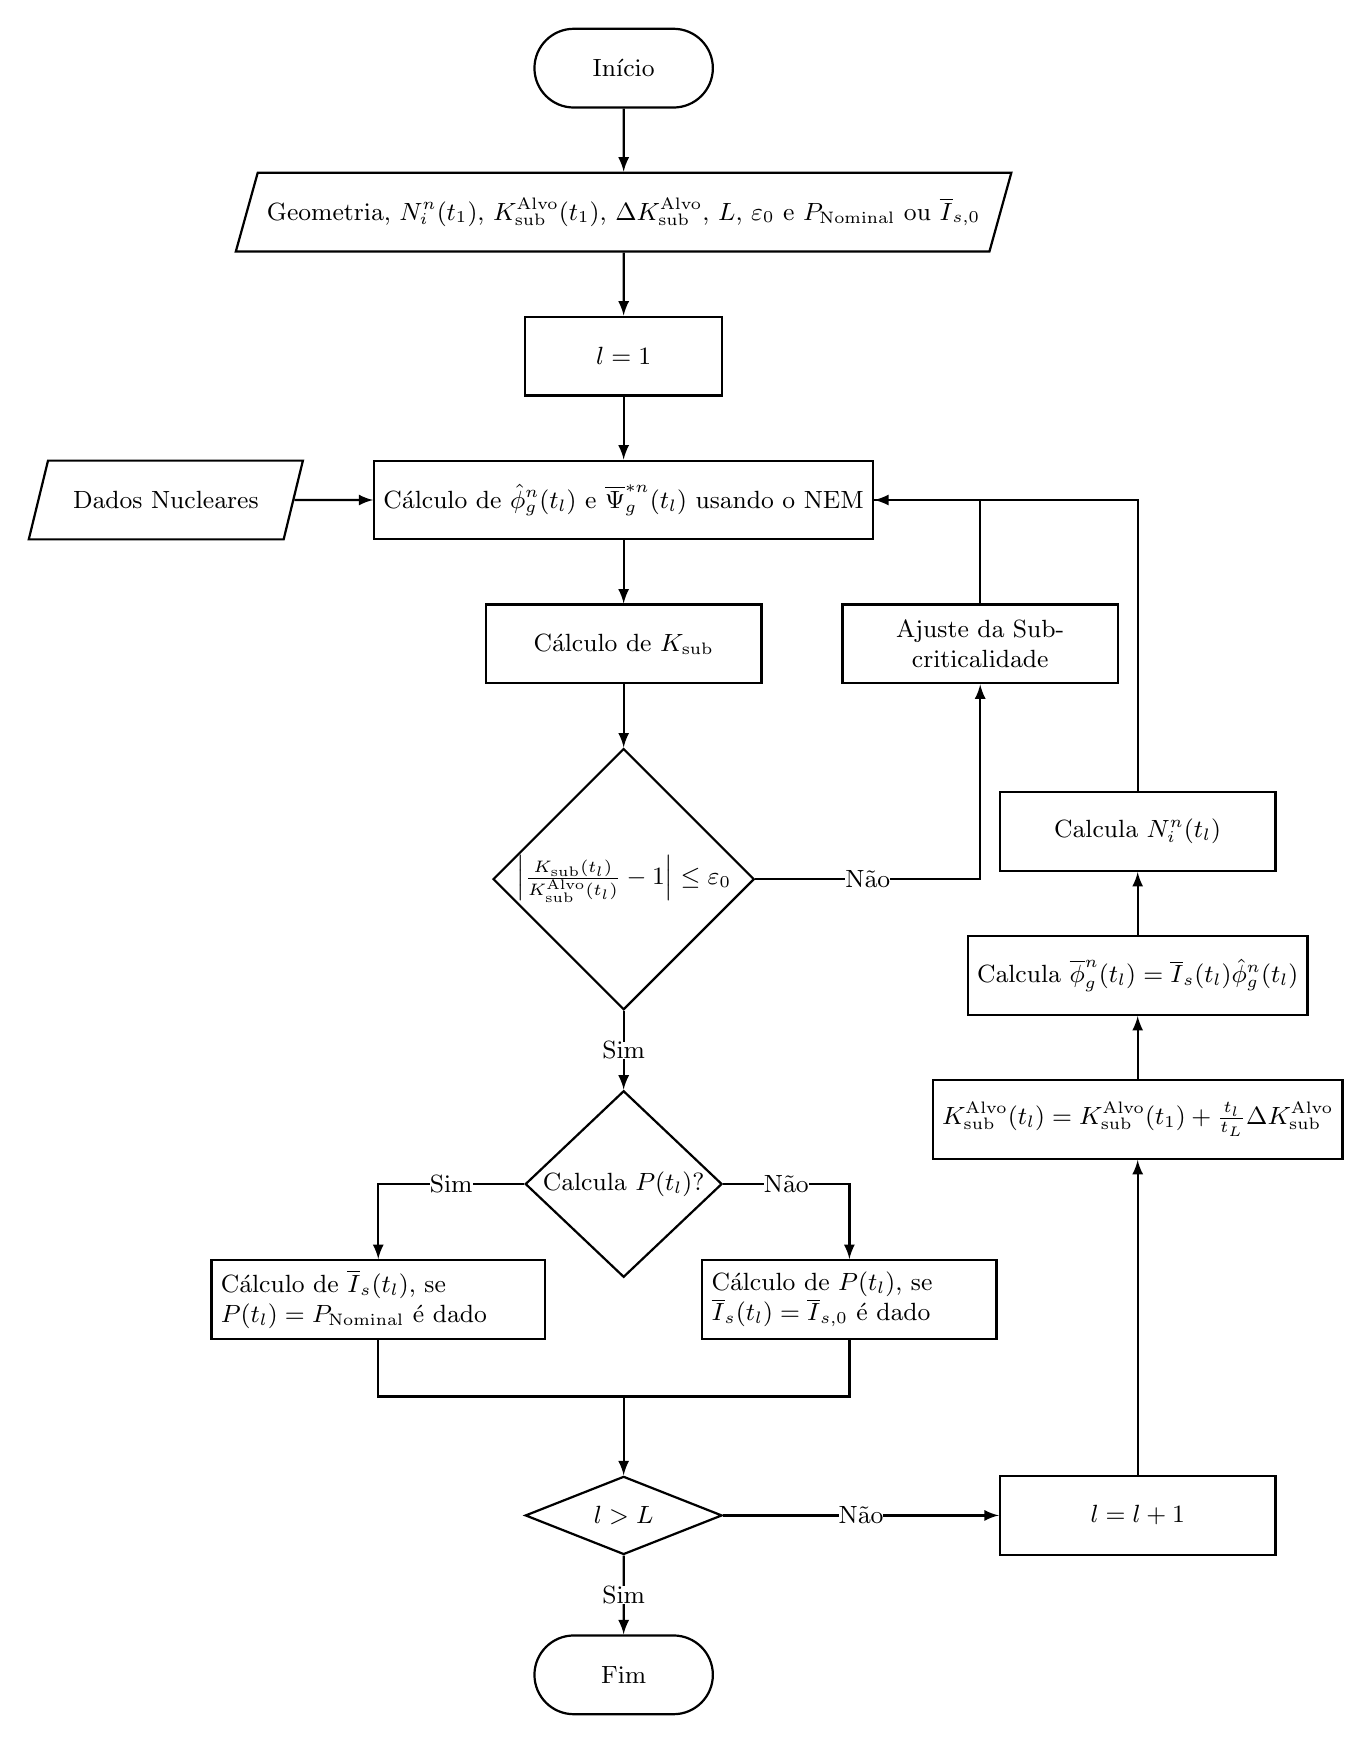
\begin{tikzpicture}[font=\small,thick]
 
% Start block
\node[draw,
    rounded rectangle,
    minimum width=2.5cm,
    minimum height=1cm] (block1) {Início};
 
% Voltage and Current Measurement
\node[draw,
    trapezium, 
    trapezium left angle = 65,
    trapezium right angle = 115,
    trapezium stretches,
    below= 0.8cm of block1,
    minimum width=3.5cm,
    minimum height=1cm
] (block2) { Geometria, $N_i^n{(t_1)}$, $K_{\text{sub}}^\text{Alvo}(t_1)$, $\Delta K_{\text{sub}}^\text{Alvo}$, $L$, $\varepsilon_0$ e $P_\text{Nominal}$ ou $\overline{I}_{s,0}$};
 
% Power and voltage variation
\node[draw,
    below=0.8cm of block2,
    minimum width=2.5cm,
    minimum height=1cm
] (block3) { $l=1$};

% Power and voltage variation
\node[draw,
    below=0.8cm of block3,
    minimum width=3.5cm,
    minimum height=1cm
] (block4) {Cálculo de $\hat{\phi}_g^n(t_l)$ e $\overline{\Psi}_g^{*n}(t_l)$ usando o NEM};

% Voltage and Current Measurement
\node[draw,
    trapezium, 
    trapezium left angle = 65,
    trapezium right angle = 115,
    trapezium stretches,
    left=of block4,
    minimum width=3.5cm,
    minimum height=1cm
] (block21) {Dados Nucleares};

% Power and voltage variation
\node[draw,
    below=0.8cm of block4,
    minimum width=3.5cm,
    minimum height=1cm
] (block5) {Cálculo de $K_{\text{sub}}$};
    
% Conditions test
\node[draw,
    diamond,
    below=0.8cm of block5,
    minimum width=2.5cm,
    inner sep=0] (block6) {$\left|\frac{K_{\text{sub}}(t_l)}{K_{\text{sub}}^\text{Alvo}(t_l)} -1 \right| \le \varepsilon_0$};
    
    
% Conditions test
\node[draw,
    diamond,
    below=of block6,
    minimum width=2.5cm,
    inner sep=0] (block7) {Calcula $P(t_l)$?};   

% Power and voltage variation
\node[draw,
    below left=0.5cm of block7,
    minimum width=3.5cm,
    minimum height=1cm,
    text width=4cm
] (block8) {Cálculo de $\overline{I}_s(t_l)$, se $P(t_l)=P_\text{Nominal}$ é dado};  

% Power and voltage variation
\node[draw,
    below right=0.5cm of block7,
    minimum width=3.5cm,
    minimum height=1cm,
    text width=3.5cm
] (block9) {Cálculo de $P(t_l)$, se $\overline{I}_s(t_l)=\overline{I}_{s,0}$ é dado};  

% Power and voltage variation
\node[draw,
    right= 1cm of block5,
    minimum width=3.5cm,
    minimum height=1cm,
    text width=3cm,
    text centered
] (block17) {Ajuste da Subcriticalidade};  

\node[coordinate,below=1.5cm of block7] (block16) {};

% Conditions test
\node[draw,
    diamond,
    below= of block16,
    minimum width=2.5cm,
    inner sep=0] (block10) {$l>L$};
  

%\node[coordinate,right=0.5cm of block17] (block18) {};
    

% Power and voltage variation
\node[draw,
    right=3.5cm of block10,
    minimum width=3.5cm,
    minimum height=1cm
] (block12) {$l=l+1$};

% Power and voltage variation
\node[draw,
    above=4cm of block12,
    minimum width=3.5cm,
    minimum height=1cm
] (block13) {$K_{\text{sub}}^\text{Alvo}(t_l) = K_{\text{sub}}^\text{Alvo}(t_1) + \frac{t_l}{t_L}\Delta K_\text{sub}^\text{Alvo}$}; 

% Power and voltage variation
\node[draw,
    above=0.8cm of block13,
    minimum width=3.5cm,
    minimum height=1cm
] (block14) {Calcula $\overline{\phi}_g^n(t_l) = \overline{I}_s(t_l)\hat{\phi}_g^n(t_l)$};    


% Power and voltage variation
\node[draw,
    above=0.8cm of block14,
    minimum width=3.5cm,
    minimum height=1cm
] (block18) {Calcula $N_i^n(t_l)$};    
    
% Return block
\node[draw,
    rounded rectangle,
    below=of block10,
    minimum width=2.5cm,
    minimum height=1cm,] (block11) {Fim};
 
% \node[coordinate,below=4.35cm of block4] (block12) {};
 
 
% Arrows
\draw[-latex] (block1) edge (block2)
    (block2) edge (block3)
    (block3) edge (block4)
    (block21) edge (block4)
    (block4) edge (block5)	
    (block5) edge (block6);
 
\draw[-latex] (block6) -- (block7)
    node[pos=0.5,fill=white,inner sep=0]{Sim};
    
\draw[-latex] (block6) -| (block17)
    node[pos=0.25,fill=white,inner sep=0]{Não};    
 
\draw[-latex] (block7) -| (block8)
    node[pos=0.25,fill=white,inner sep=0]{Sim};

\draw[-latex] (block7) -| (block9)
    node[pos=0.25,fill=white,inner sep=0]{Não};

\draw (block8) |- (block16);
 
\draw (block9) |- (block16);

\draw[-latex] (block16) -- (block10);

\draw[-latex] (block10) -- (block11)
    node[pos=0.5,fill=white,inner sep=0]{Sim};

\draw[-latex] (block10) -- (block12)
    node[pos=0.5,fill=white,inner sep=0]{Não};


\draw[-latex] (block12) edge (block13)
              (block13) edge (block14)
              (block18) |- (block4)
              (block17) |- (block4)
              (block14) edge (block18);
%\draw (block17) -- (block18);              
 
\end{tikzpicture}
\vspace{-1cm}
\caption{Fluxograma do algoritmo de solução para determinar o parâmetro $K_{\text{sub}}$.}
\label{chap3:fluxograma}
\end{figure}

    \chapter{Frapi v2: back-end design guidelines}
\label{chap4}

Read-only endpoints built with Frapi and the FracTree ORM are not difficult to maintain. One JSON per resource exposed by the API is sufficient. The scenario changes when dealing with write operations due to new factors of data validation, communication with external systems, business rules checks and modelling of the problem domain.
Frapi class-based custom routes were created as a temporary solution for write operations and were not ideal.

The \texttt{buildEndpoints()} method of endpoint classes is completely flexible, allowing the API developer to design the back end as wanted. This feature became an issue. Frapi applications with similar use cases and the same technology stack were being developed ad-hoc, with diverse standards and code organisation. It was harder for developers from different projects to help teammates due to different setups and ways to solve the same problems.

Used to the ``FENCE way'' of writing programs, the Glance Team started to repeat the same mistakes made on the old framework systems. The learning curve was still something to be aware of. There was a high coupling between new components, a lack of tests and common infrastructure problems were being solved by the team instead of relying on third-party solutions. To avoid migrating the applications to another solution and keeping the same problems, a task force was created to study how the back end was designed in the software industry and propose a series of guidelines to be followed by Frapi systems. The proposed structure should, thus, be strict in the way that multiple applications use the same patterns and are flexible enough to be extended according to the system's needs.

Therefore, Frapi v2 is essentially a shift in how REST APIs are developed using the FENCE module by adding the \textit{controller} endpoint type described in \autoref{sec:controller-endpoints}. The shared structure inspirations, design guidelines and how to apply them will be discussed in depth in the remaining sections.

\section{Controller endpoints}
\label{sec:controller-endpoints}

Controller endpoints are a new way of defining REST API routes on Frapi with the goal of replacing \textit{class endpoints} (\autoref{sec:custom-endpoints}) and solving some of its issues. The previous alternative used direct access to the Slim micro-framework for routing inside the \texttt{buildEndpoints()} function. It created a discrepancy of where routes were registered, \textit{FacTree endpoints} were defined on JSON files while \textit{class endpoints} were defined on PHP classes, usually in different directories, decreasing general maintainability and difficulting for new developers to read the API source code. The direct access to Slim bypassed the abstraction created by Frapi, making future replacements and updates of the framework more difficult and thus affecting the system's extensibility and adding the risk of accumulating technical debt.

\subsection{Route definitions}

To keep consistency with \textit{FacTree endpoints}, the endpoint path and method are configured in JSON files. \nameref{code:controller-endpoint-json} illustrates the configuration of controller endpoints for the Service Work task resource. By defining the \texttt{controller} type and specifying the class, Frapi will instantiate it and call the configured methods according to the received request. Routes are defined under the texttt{paths} parameter, where keys are the URI paths of the endpoints, and the values contain another set of keys corresponding to the HTTP method. The \texttt{method} configuration defines the method of the controller class that will be called when the request is received.

\begin{listing}[htbp]
\begin{minted}{json}
{
    "type": "controller",
    "class": "\\Alice\\ServiceWork\\TaskController",
    "paths": {
        "/tasks": {
            "GET": { "method": "findAllTasks" },
            "POST": { "method": "registerTask" }
        },
        "/tasks/:id": {
	        "GET": { "method": "findTask" },
            "PUT": { "method": "updateTask" },
            "DELETE": { "method": "removeTask" }
        }
    }
}
\end{minted}
\caption{Route definitions of controller-based endpoints.}
\label{code:controller-endpoint-json}
\end{listing}

Following the example, if a client sends a \texttt{GET /tasks} request, Frapi will instantiate a \texttt{Alice\textbackslash ServiceWork\textbackslash TaskController} object and call the \texttt{findAllTasks} method. Observe how multiple routes are registered in an organised and readable manner, helping the developer easily view the available endpoints and which method is executed when they are requested.

The controller class is shown on \nameref{code:controller-endpoint-php}. The controller methods should be public and have an \texttt{Api} object as the first argument, which could be used to get the request and the response objects. The response must be returned at the end of the method to be sent to the client.

\begin{listing}[htbp]
\begin{minted}{php}
<?php

namespace Alice\ServiceWork;

use Fence\Frapi\Api;
use Fence\Frapi\Response;

class TaskController
{
	public function findAllTasks(Api $api): Response
	{
		$request = $api->getRequest();
		// Find task...
		
		$response = $api->getResponse();
		// Write response...

		return $response;
	}

	public function removeTask(Api $api, $id): Response
	{
		// Remove task by ID...
	}

	// Other methods...
}
\end{minted}
\caption{Controller class that handles Service Work task-related requests.}
\label{code:controller-endpoint-php}
\end{listing}

The \nameref{code:controller-endpoint-json} and \nameref{code:controller-endpoint-php} also exemplify how parameters can be used on the URI. In the case of deleting the task with ID 197, it is a common practice in REST APIs to send a request similar to \texttt{DELETE /tasks/197}. Frapi supports this scenario by following the Slim v2 convention \cite{slim-v2-routing-params} with the \texttt{:id} parameter on the endpoint path, which will be used when calling the controller method \texttt{removeTask}.

\subsection{Authorisation}

Controller endpoints also support access control. To protect a route, a permission schema should be added under the \texttt{authorization} key. The authorisation mechanism is identical to the one used by the first version of Frapi on the FacTree endpoints (\autoref{sec:frapi-v1-authorisation}).

\begin{listing}[htbp]
\begin{minted}{json}
{
    "type": "controller",
    "class": "\\Alice\\ServiceWork\\TaskController",
    "paths": {
        "/tasks": {
            "POST": {
	            "method": "registerTask",
	            "authorization": [
                    { "roles": ["admin"] }
                ]
	        }
        },
    }
}
\end{minted}
\caption{Authorisation configuration for controller-based endpoint.}
\label{code:controller-endpoint-auth-json}
\end{listing}

\subsection{Request validation}

To address a shared need between applications to guarantee a correctly formatted HTTP request body, the feature of schema-based validation was introduced to Frapi. The solution consists of checking the requests body JSON against a schema with rules of expected keys, values types and formats, and optional fields defined in the already established JSON Schema standard \cite{json-schema-spec}.

Following the specification, schemas are written in JSON format. Since they usually contain multiple lines of rules and definitions, the design decision was to create a file for each schema. Each is referenced on the controller endpoint file under the \texttt{schema} key as exemplified on \autoref{code:controller-endpoint-schema-json}.

\begin{listing}[htbp]
\begin{minted}{json}
{
	"type": "controller",
    "class": "\\Alice\\ServiceWork\\TaskController",
    "paths": {
		"POST": {
                "method": "registerTask",
                "schema": "resources/schemas/task-register.json"
            }
        }
    }
}
\end{minted}
\caption{Request validation configuration for controller-based endpoint.}
\label{code:controller-endpoint-schema-json}
\end{listing}

\subsection{Dependency injection}
\label{sec:dependency-injection}

Following the example on \autoref{code:controller-endpoint-schema-json}, Frapi internally instantiates the \texttt{TaskController} class and calls the \texttt{registerTask} method as simplified on \autoref{code:controller-call}. The controller instantiation is trivial when it does not have any dependencies.

\begin{listing}[htbp]
\begin{minted}[startinline]{php}
$controller = new \Alice\ServiceWork\TaskController();
$controller->registerTask($api);
\end{minted}
\caption{Controller class instantiation.}
\label{code:controller-call}
\end{listing}

Take \autoref{code:controller-with-dependencies} as an example, which uses the dependency injection (DI) \cite{php-the-right-way-di} pattern, which removes hard-coded dependencies, making it possible to replace them as desired. The controller has two dependencies (database connection and email service) at the constructor level which Frapi would need to resolve somehow similar to \autoref{code:controller-with-dependencies-call}. Without any hints, it is not possible for Frapi to instantiate the dependencies, and also their own dependency tree, to call the controllers.

\begin{listing}[htbp]
\begin{minted}[startinline]{php}
class TaskController
{
	public function __constructor(
		DatabaseConnection $connection,
		EmailService $emailService
	) {
	}

	public function registerTask(Api $api): Response
	{
		// Use database connection and email service
		// to register a task...
	}
}
\end{minted}
\caption{Controller class with dependencies.}
\label{code:controller-with-dependencies}
\end{listing}

\begin{listing}[htbp]
\begin{minted}[startinline]{php}
$connection = new DatabaseConnection($dsn, $user, $password);
$emailService = new EmailService($credentials);
$controller = new TaskController($connection, $emailService);
\end{minted}
\caption{Manual instantiation of the controller class.}
\label{code:controller-with-dependencies-call}
\end{listing}

To address the need for automatically injecting dependencies, the second version of Frapi introduced support for DI containers. The container is a tool to make the injection more practical by letting the application define how classes and interfaces should be created and by instantiating and injecting them. It was decided not to rely on any specific third-party tool but instead use PSR-11 \cite{psr-11} containers. PHP Standard Recommendations (PSRs) are a set of interfaces created by the Framework Interoperability Group (FIG) \cite{fig-website} to standardise the commonalities between established PHP projects. All the major PHP DI container libraries follow the container interface from PSR-11, allowing Frapi applications to choose between a wide range of tools according to their needs.

Frapi uses the DI container provided by the application to create the controllers. The container is sent to Frapi via the texttt{setContainer()} method as shown on \autoref{code:set-container-example}. PHP-DI \cite{php-di} is used in the example, but any other PSR-11 container could be used.

\begin{listing}[htbp]
\begin{minted}[startinline]{php}
$containerBuilder = \DI\ContainerBuilder();
$containerBuilder->addDefinitions([
	DatabaseConnection::class => function () {
		return new DatabaseConnection(
			getenv(DB_CONNECTION_STRING),
			getenv(DB_USERNAME),
			getenv(DB_PASSWORD)
		);
	},
	EmailService::class => function () {
		return new EmailService(getenv("EMAIL_CREDENTIALS"));
	},
]);
$container = $containerBuilder->build();

$api = new Api("configuration.json");
$api->setContainer($container);

$api->run();
\end{minted}
\caption{Dependency injection definitions and usage example of the \texttt{setContainer} method.}
\label{code:set-container-example}
\end{listing}

\section{Framework independence}

The remaining sections will no longer describe Frapi features and internal behaviour but instead focus on creating guidelines to design better and set standards for back ends across the Glance Team due to common problems and use cases. The individualities of each project were also kept in mind, resulting in the need for flexible guidelines.

At this point, the bottleneck of development speed and maintenance created by FENCE was well-known around the team. The first decision of the guidelines was to not rely heavily on a framework. Frameworks help create simple CRUD applications rapidly and have large communities, providing a significant amount of support and documentation. However, their generalist nature conflicts with the need to create systems with complex rules. What at first was a tool which enabled fast bootstrapping became an obstacle for developers to evolve the application around the framework.

Notice that frameworks were not banned. Applications could use them but were strongly advised to avoid using external libraries at the core of their projects. Regarding FENCE, the team decided to avoid almost everything from the in-house and use external libraries for common problems. Since Frapi was packed inside FENCE, its usage was allowed. The Logger was inspired by PSR-3 \cite{psr-3} and could be replaced without much work. It was discouraged the usage of other classes and features from FENCE, such as \texttt{Configuration}, FacTree models and \texttt{Utils}.

\section{Domain-Driven Design}
\label{sec:ddd}

Frapi applications started as an interface to external systems to consume Glance data. With the decision to develop applications with decoupled front-end and back-end layers, REST APIs would need to handle all read-and-write use cases. It was already known that the new projects would not have to deal with simple CRUD operations but would need to implement all the complex business rules and processes unique to the collaboration of each experiment. Based on the problems of creating purely in-house solutions and developing ad-hoc, the team researched to find existing patterns which could be used as a base for building complex software systems.

Domain-Driven Design (DDD) was the main inspiration for the back-end guidelines. It is a set of principles initially defined in the book \textit{Domain-Driven Design: Tackling Complexity in the Heart of Software} written by Eric Evans in 2003 \cite{ddd-blue-book}. The author proposes developing software solutions centred on the domain model with a great understanding of the rules and flows of the business. It fits the needs of systems similar to the ones built by Glance Team, which provide solutions to complex domains with messy logic to be organised \cite{ddd-martin-folwer}. Since the first publication, the principles gained adoption, were put into practice and evolved. The methodology became particularly popular among microservices, helping to split a system into smaller services by identifying the responsibilities and relations of each.

The DDD methodology is divided into two phases: Strategic and Tactical Design. The former involves a deep understanding of the business and defining responsibilities and boundaries among modules. It should answer \textit{what} and \textit{why} is the software solution being built. The latter focuses on \textit{how} to translate the knowledge extracted from the first phase into code by defining building blocks. The blocks, such as entities, value objects, aggregates, services, repositories, and events, will be explained briefly on \autoref{sec:building-blocks}. For an in-depth explanation of each pattern, it recommended the read of Evans' original text \cite{ddd-blue-book} and Vaughn Vernon's \textit{Implementing Domain-Driven Design} book \cite{ddd-red-book}.

The Strategic Design suggests breaking the domain, which may be broad and abstract, into smaller pieces called \textbf{subdomains} \cite{petter-holmstrom-part1}. Subdomains can be classified as \textbf{core}, \textbf{supporting}, and \textbf{generic}. Core subdomains are the most important, special and unique parts of the domain. They are the reason for the existence of the system. Generic subdomains are the pieces that are unrelated to the organisation and can be replaced by third-party solutions but are still needed for the operation of the overall solution. Supporting subdomains are the ones which are not part of the main goal of the solution but are also not generic enough since they require specific context about the organisation. For example, on the Service Work system, the ALICE task management domain was split into seven subdomains as illustrated on \autoref{fig:sw-subdomains-diagram}. The \textit{Task} subdomain encompasses the management of tasks, including planning and assignments. It is categorised as core because it is vital to Service Work. \textit{Institutions} is an example of a supporting subdomain. It includes the modelling of institutes, clusters and service clusters of the ALICE collaboration, containing specific knowledge of the domain but not being its core. Finally, generic subdomains are exemplified by \textit{Identity and Access} and \textit{Notification}. Both parts do not contain any logic unique to CERN, ALICE or Service Work and could be replaced by off-the-shelf solutions but are essential for the overall workflow of the system.

\begin{figure}[htbp]
  \centering
  \includesvg[scale=0.8]{Imagens/chap04/sw-subdomains-diagram.svg}
  \caption{Subdomains of the Service Work problem space.}
  \label{fig:sw-subdomains-diagram}
\end{figure}

Evans \cite{ddd-blue-book} also advocates the use of \textbf{ubiquitous language}. It is a language shared by developers and domain experts to describe the problem and the solution. Most of this language comprises the terminology used by the business or in the ALICE experiment following the Service Work example. The idea behind this concept is also to use this language to model the solution and write the software, thus reducing the communication barrier of translating technical code to domain processes.

Moving to the solution space, Domain-Driven Design also defines the concept of \textbf{bounded contexts}. Like subdomains, bounded contexts are parts of the domain, the difference being that the latter corresponds to a division on the solution space instead of the problem space. Usually, there is a one-to-one mapping between subdomains and bounded contexts, but this is not a rule. It is possible to have a single subdomain with multiple bounded contexts and vice-versa.

Understanding, discovering, decomposing and organising subdomains is not trivial and requires a deep knowledge of the entire problem space. It is crucial to first understand the problem before trying to solve it, turning communication with domain experts of great importance. Multiple techniques exist to help developers and experts visually and collaboratively map the domain \cite{ddd-modelling-process}. The exploration of the Service Work domain was done using the Event Storming \cite{event-storming-website} \cite{introducing-event-storming} approach. It consists of a brainstorm of domain \textbf{events}. An event is something meaningful that happened on the domain and is represented by orange sticky notes (see \autoref{fig:event-storming-sw-zoom-in}). Later, the \textbf{commands} that triggered the events blue notes are added before the events and with yellow notes representing the \textbf{actor} who performed the action. Finally, the sticky notes are rearranged and linked through arrows indicating that a command is triggered due to an event. If there is a condition to continue the workflow, it is represented as a purple after the event note.

\begin{figure}[htbp]
  \centering
  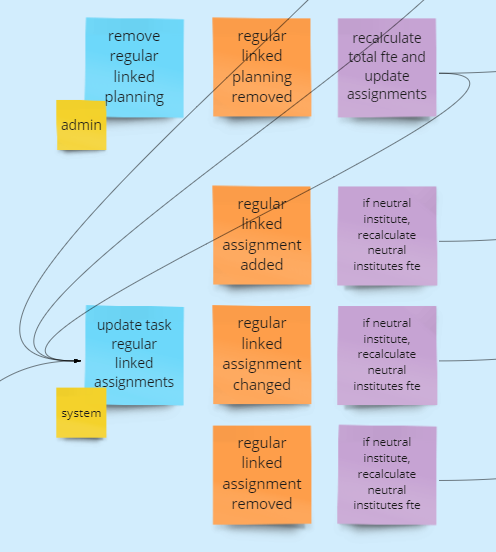
\includegraphics[scale=0.7]{Imagens/chap04/event-storming-sw-zoom-in.png}
  \caption{Details of the event storming board from Service Work.}
  \label{fig:event-storming-sw-zoom-in}
\end{figure}

Using Event Storming at Service Work facilitated the strategic design of the system. The approach helped discover events, use cases, user personas, and separation of subdomains and made it easier to visualise the various complex flows of the system. \autoref{fig:event-storming-sw-zoom-out} illustrates part of the result of event storming. Note how events were organised, permitting to draw the boundaries of the two core subdomains.

\begin{figure}[htbp]
  \centering
  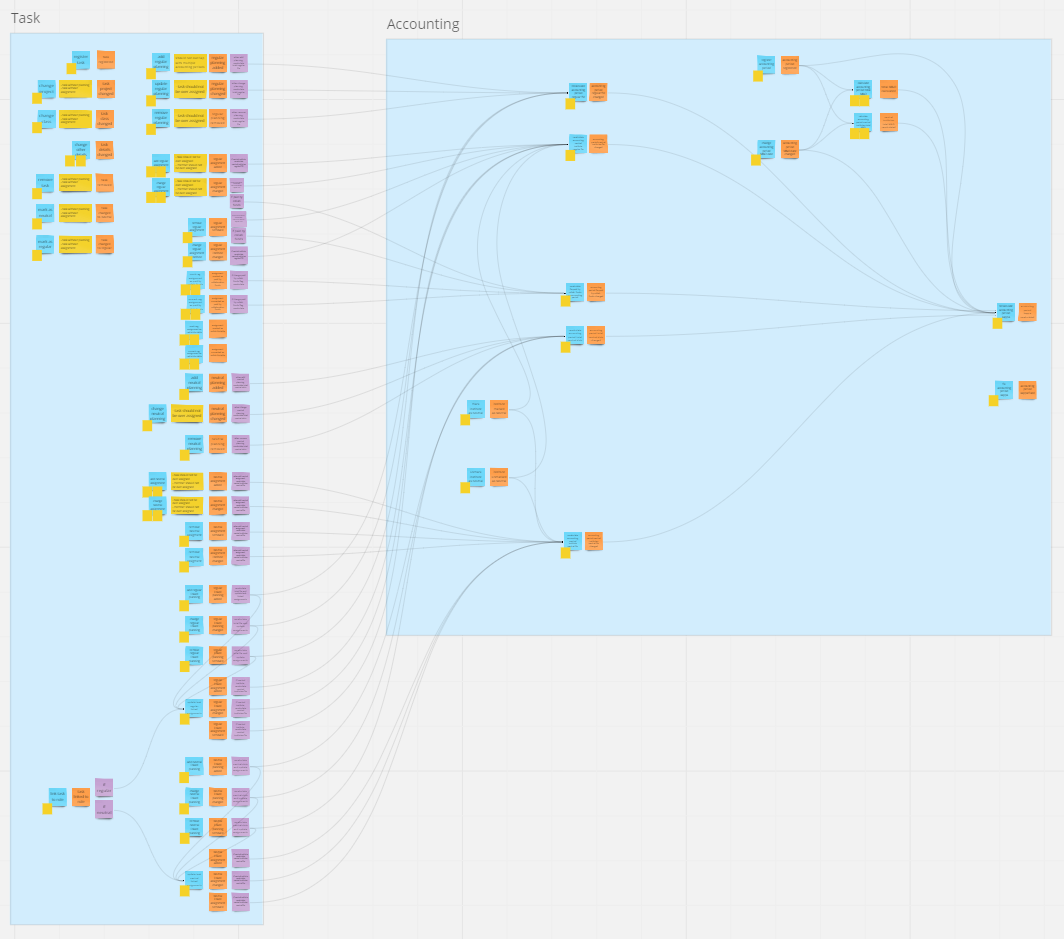
\includegraphics[scale=0.5]{Imagens/chap04/event-storming-sw-zoom-out.png}
  \caption{Part of the result of event storming at Service Work.}
  \label{fig:event-storming-sw-zoom-out}
\end{figure}

\section{Architecture}

Software architecture can be defined as the division of the system into smaller units, the relation between those components, their characteristics and how they are arranged \cite{sven-woltmann-hexagonal-architecture}. When the Glance Team started to create decoupled applications, the developers agreed that the chosen architecture must facilitate system changes. The addition or replacement of business rules, modernisation of technologies and infrastructure upgrades should be done with little and predictable effort, with explicit consequences and no hidden side effects. This characteristic should be kept up in the software during its lifetime. In other words, the Glance applications would need to be operational and maintainable for at least 20 years, during which the LHC experiments are planned to run \cite{lhc-end-of-life}.

\subsection{Layered Architecture}
\label{sec:layered-architecture}

At the beginning of the development of the first Frapi-based REST APIs, the Glance Team adopted the \textit{Layered Architecture}. Also known as \textit{n-tiered}, this architectural style organises the system components in horizontal layers with distinct roles. It mostly adopted with the \textbf{presentation}, \textbf{business}, \textbf{persistence} and \textbf{database} layers, but there is no limitation in the number and type of layers \cite{richards-architecture}. \autoref{fig:layered-architecture-on-frapi} exemplifies how Layered Architecture was used where the blue containers represent the deployable units, layers are represented in orange with their components in green. The presentation layer was responsible for handling the communication with the API consumers. \textbf{Controller} classes would parse HTTP requests, coordinate the call of business logic and later format responses. The business layer executes a \textbf{Service} with specific domain rules and flows without validating the input from the users since this is the responsibility of the previous layer. Similarly, it does not have to know how to retrieve the data and reconstruct an \textbf{Entity} since it is the responsibility of the \textbf{Repository} on the persistence layer, which communicates with the datastore on the database layer. Each layer could be tested in isolation by mocking components and other layers, facilitating the development of automated tests.

\begin{figure}[htbp]
  \centering
  \includesvg[scale=0.8]{Imagens/chap04/layered-architecture-on-frapi.svg}
  \caption{Layered architecture diagram.}
  \label{fig:layered-architecture-on-frapi}
\end{figure}

Due to its simplicity, the Layered Architecture has low development cost and is well suited for small and simple applications. However, as the Glance APIs increased their inherent complexity, maintainability was affected. By being technically partitioned, components were grouped by their technical function instead of their business role \cite{richards-architecture}. It became challenging to reason about the complex domain constraints and processes when everything was partitioned on the same layer. The style also induces developers to a data-driven design, with the software being built around how the database is structured and the relation between tables. By focusing on how data is persisted instead of modelling the business and its behaviour, the approach moved away from the desired domain-driven design.

\subsection{Hexagonal Architecture}
\label{sec:ports-and-adapters}

With the downsides of Layered Architecture, the team went back to research a new architectural style that would better fit with domain-driven design due to the business complexity of the systems. The chosen solution was the \textit{Ports and Adapters Architecture}, also known as \textit{Hexagonal Architecture}, proposed by Alistair Cockburn in 2005 \cite{alistair-cockburn-hexagonal-architecture}. It defends that the business logic should be developed in isolation, allowing the system to be equally used by users, external services and test runners. The use cases and business logic are encapsulated at the core of the architecture called \textbf{application} as illustrated on \autoref{fig:ports-and-adapters-diagram}. On this layer, \textbf{ports} serve as an interface to external components such as users, REST API clients, databases, filesystem and third-party APIs. The connection with the outside world is made on the outer layer of the hexagon via \textbf{adapters}, which implement the port interfaces. \textit{Driving} ports and adapters control the application are represented on the left side of the diagram, while the \textit{driven} components are placed on the right side \cite{sven-woltmann-hexagonal-architecture}. The style defined by Cockburn is almost identical to Robert Martin's \textit{Clean Architecture} \cite{robert-martin-clean-architecture-book} and Jeffrey Palermo's \textit{Onion Architecture} \cite{onion-architecture-article}.

\begin{figure}[htbp]
  \centering
  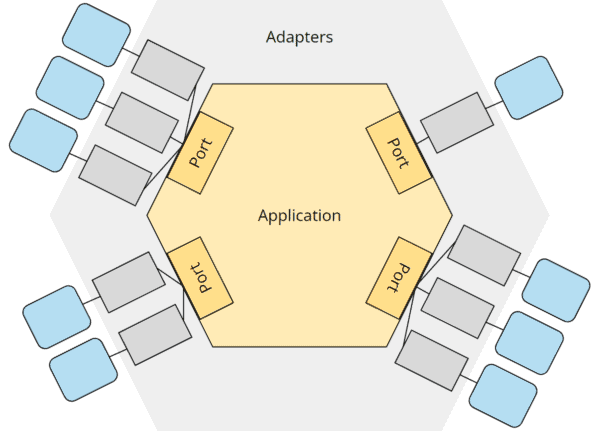
\includegraphics[scale=0.5]{Imagens/chap04/ports-and-adapters-diagram.png}
  \caption{Ports and adapters components on the hexagonal architecture \cite{sven-woltmann-hexagonal-architecture}.}
  \label{fig:ports-and-adapters-diagram}
\end{figure}

Note how the control of the system on this architecture flows from left to right: it starts on the driving components, going to the corresponding adapters and ports, calling the business logic which then uses the driven components by using their corresponding ports implemented by adapters. The source code dependency, however, is different, as shown on the left diagram of \autoref{fig:hexagonal-architecture-vs-layered-architecture-diagrams}. All the components of this architecture depend on their current or inner layers. The business is the central part, everything depends on it, but the domain code has no dependencies, turning it technically simple and allowing it to focus on modelling the complex business. This dependency characteristic facilitates the domain-driven design approach in contrast with the Layered Architecture in which the components' dependencies points to the database layer, as illustrated on the right diagram of \autoref{fig:hexagonal-architecture-vs-layered-architecture-diagrams}.

\begin{figure}[htbp]
  \centering
  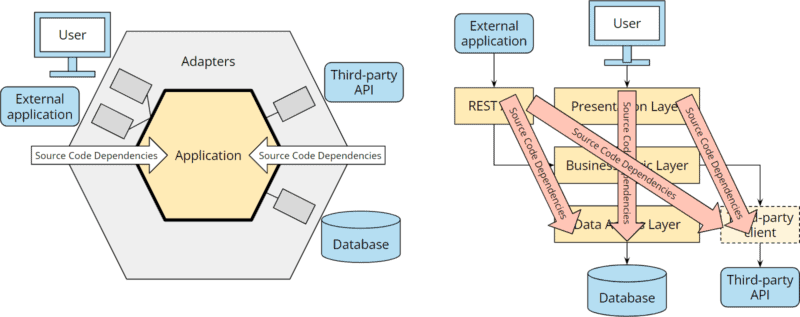
\includegraphics[scale=0.5]{Imagens/chap04/hexagonal-architecture-vs-layered-architecture-diagrams.png}
  \caption{Comparison between \textit{Ports and Adapters} and \textit{Layered} architectures \cite{sven-woltmann-hexagonal-architecture}.}
  \label{fig:hexagonal-architecture-vs-layered-architecture-diagrams}
\end{figure}

The Ports and Adapters Architecture allows easy modifying or even replacing adapters. This is an advantage since it brings the possibility of changing infrastructure components such as databases, upgrading dependencies, and also performing tests by using mock adapters without much effort. Another benefit of Hexagonal Architecture is that the team can start developing and modelling the domain code without having to know about what infrastructure components will be used, such as frameworks and database types, and delaying this decision to a later stage with a mature project and a clearer vision of the system needs \cite{sven-woltmann-hexagonal-architecture}.

\subsection{Modular Monolith}
\label{sec:modular-monolith}

To avoid the issues of a technically partitioned exposed on \autoref{sec:layered-architecture}, the Glance Team decided to divide the system in bounded contexts (\autoref{sec:ddd}), reflecting the subdomains of the problem space. Contexts are independent modules and follow the Ports and Adapters architectural style. \autoref{fig:multiple-bounded-contexts} illustrates this topology with three bounded contexts, each represented by a hexagon. Each module can consume data from databases, external APIs and even other internal models. As a guideline, modules should not directly depend on other bounded context components but instead make use of ports and adapters. 

\begin{figure}[htbp]
  \centering
  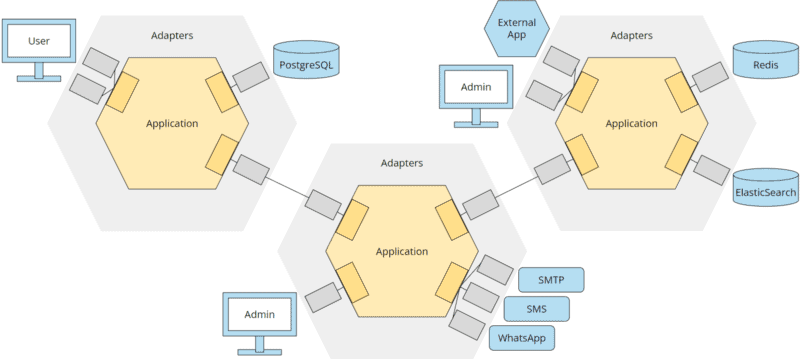
\includegraphics[scale=0.5]{Imagens/chap04/multiple-bounded-contexts.png}
  \caption{Multiple bounded contexts on the hexagonal architecture \cite{sven-woltmann-hexagonal-architecture}.}
  \label{fig:multiple-bounded-contexts}
\end{figure}

Even though the Hexagonal Architecture is well suited for distributed microservices, the Glance Team agreed to use at first a \textbf{monolithic topology}. The nonfunctional characteristics of distributed computing, such as performance, scalability and availability, were not typical requirements for the projects being developed. Creating multiple deployable units would bring unnecessary technical complexity and other groups of issues, such as the fallacies of distributed computing, described by Peter Deutsch and James Gosling in 1994 and 1997 \cite{fallacies-of-distributed-computing} \cite{richards-architecture}. The benefits of microservices for big teams were also not applicable since the development teams for each Glance system are usually from one to three members.

Unlike a classic monolith such as FENCE systems, the proposed topology is a \textbf{modular monolith}. The system comprises modules (bounded contexts) forming a single deployable package. Contexts do communicate with each other internally on the same thread and programming language (PHP) by using ports and adapters as if they were distributed to avoid high coupling. It is also possible to perform internal communication via REST API requests, but this is unnecessary, resulting in a loss of performance without any gain.

The same reasons for not using microservices apply to databases. A common solution may use one persistence mechanism per module to isolate data. For simple deployments, easy maintenance and considering the low number of developers, the Glance team decided to use at first one database per system. It could be split into several databases if needed in the future. To preserve data isolation, the database may be divided logically by bounded context, for example, by adding a module prefix to each table name and discouraging the usage of tables from outside the module.

\autoref{fig:service-work-topology} illustrates a simplified version of the Service Work system topology. It is composed of four deployable units in blue: \textit{front end}, \textit{back end}, \textit{database} and \textit{job scheduler}. The back end is an example of a modular monolith composed of seven bounded contexts reflecting the subdomains of the business (\autoref{fig:sw-subdomains-diagram} on \autoref{sec:ddd}). Modules communicate internally with each other and also use external resources such as the database, third-party APIs (CERN Authorization Service) and legacy systems. In this case, the Membership bounded context works as an anticorruption layer \cite{ddd-blue-book} to access a legacy system. Observe how the database is logically divided into parts used only by their corresponding modules. Clients like the front and external systems can call the back end via HTTP, while the job scheduler uses a command line interface.

\begin{figure}[htbp]
  \centering
  \includesvg[scale=0.65]{Imagens/chap04/service-work-topology.svg}
  \caption{The modular monolith topology of the Service Work system.}
  \label{fig:service-work-topology}
\end{figure}

\section{Building blocks}
\label{sec:building-blocks}

The current section describes recommended building blocks for implementing Glance REST APIs. As the entire guideline, this is not a definitive list with immutable rules. Exceptions can exist, and better ways of developing complex applications may be proposed. The blocks are patterns and best practices from object-oriented programming and may be found in the literature with different names depending on the reference. On the DDD scope, they are divided into three layers: \textbf{domain}, \textbf{application} and \textbf{infrastructure}. 

\subsection{Domain}

Domain objects are used to model the business and express its logic. This layer consists of simple and isolated classes without dependency on infrastructure, user interface and application code. Without other responsibilities, domain objects can focus purely on reflecting all the nuances of the problem space with rich detail on all essential constraints, behaviours and events.

\subsubsection{Value Object}
\label{sec:value-object}

Value objects \cite{ddd-blue-book} \cite{ddd-reference} are used to represent measurable, quantifiable values or to simply describe concepts in an easier way to test, use and maintain \cite{ddd-red-book}. These objects model the domain and care about their values instead of their identity. Take, for example, a 2-dimensional coordinate represented by points X and Y. The point (1,4) equals any other point with $X = 1$ and $Y = 4$. In this case, it makes sense to model coordinates as a value object \cite{fowler-value-objects}. On the other hand, two different individuals named ``Eric ''may not be the same person. If a person changes their name, it remains the same person. Thus their identity matters, and value objects may not be the best choice to model a person.

On Service Work, FTE (Full-Time Equivalent) represents the work planned or assigned to a task. 1 FTE is the maximum amount of work of a collaboration member. 1 FTE during one day equals 8 working hours, but 1 FTE during a week equals 40 work hours. \autoref{code:fte-example} illustrates how the application uses value objects to model a domain concept. Instead of representing FTEs as primitive float values, a class was created. Note how the domain constraint of FTEs being always positive is enforced at the constructor level. This design eliminates the need for validating this rule anywhere else in the system.

\begin{listing}[htbp]
\begin{minted}[startinline]{php}
class Fte
{
	public function __construct(
		public readonly float $value
	) {
		if ($value <= 0) {
			throw new \Exception("FTE must be positive.");
		}		
	}

	public function equals(Fte $otherFte): bool
	{
		return $this->value === $otherFte->value;
	}

	public function add(Fte $fte): Fte
	{
		$sum = $this->value + $fte->value;
		return new self($sum);
	}
}
\end{minted}
\caption{Value object to model the domain concept of FTE.}
\label{code:fte-example}
\end{listing}

Value objects can contain other value objects. Continuing the Service Work narrative, if a task is planned to have 0.5 FTEs during 6 months, a member of the ALICE collaboration should work half-time for six months to complete this task. Other combinations, such as working full-time for three months, are also possible. The \texttt{FtePeriod} class on \autoref{code:fte-period-example} illustrates how the combination of FTEs and a date period can be modelled. It enforces the domain rule that FTE periods should start and end at the corresponding month's start and end dates. It is also immutable. Any change on a value object implies the creation of a new object, preventing side effects. The immutability is exemplified by the methods \texttt{withFte} and \texttt{withPeriod}.

\begin{listing}[htbp]
\begin{minted}[startinline]{php}
class FtePeriod
{
	public function __construct(
		public readonly Period $period,
		public readonly Fte $fte,
	) {
		if (!$period->startsAtFirstDayOfMonth()) { /* ... */ }
		if (!$period->endAtLastDayOfMonth()) { /* ... */ }
	}

	public function withFte(Fte $fte): self
	{
		return new self($this->period, $fte);
	}

	public function withPeriod(Period $period): self { /* ... */ }

	/* ... */
}
\end{minted}
\caption{Value object to model the domain concept of FTE Period.}
\label{code:fte-period-example}
\end{listing}

\subsubsection{Entity}

Entities are objects defined and distinguished by their identity instead of their attributes \cite{ddd-blue-book}. Following the same example from \autoref{sec:value-object}, if a class is created to model members of the ALICE collaboration, we cannot say that two member objects with the name field “Robert” are the same because people are not fully distinguishable by their name. And if a member changes their name, it remains the same person. Even with different attributes, if two entity objects reference the same identity, they should be considered equal. Different from value objects, entities are mutable and preserve state.

Moving away from a data-centric approach, entities are not modelled with the database in mind. The idea is to create rich classes full of behaviour and domain context. Properties and methods are meaningful, with the same terms domain experts use and without technical names. The idea is to avoid an anaemic domain model \cite{ddd-blue-book} \cite{martin-fowler-anemic-domian-model} made majoritarian of getters and setters, mirroring the database table structure. Without the distractions and technicalities of frameworks, complex domain ideas become simple. The easiness of reading and reasoning about the domain allows rapid additions and changes of business rules on the code.

\autoref{code:entity-task-example} illustrates a simplification of the \texttt{Task} entity from the Service Work application. The properties consist of native PHP types (\texttt{\$name}), value objects (\texttt{\$id}) and other entities (\texttt{\$plannings} and \texttt{\$assignments}). Notice that there are no explicit getters and setters usually found on CRUD-like applications. Instead, there are domain-rich methods full of behaviour and context.

\begin{listing}[htbp]
\begin{minted}[startinline]{php}
class Task
{
	private TaskId $id;
	private string $name;
	/** @var Planning[] */
	private array $plannings;
	/** @var Assignment[] */
	private array $assignments;

	public static function register(TaskId $id, string $name): self {
        /* ... */
    }
	public function plan(FtePeriod $ftePeriod): void {
        /* ... */
    }
	public function assign(MemberId $assignee, FtePeriod $ftePeriod): void {
        /* ... */
    }
	public function unassign(AssignmentId $assignmentId): void { /* ... */ }

	public function isPlannedOnPeriod(Period $period): bool { /* ... */ }
	public function assignableFteOnPeriod(Period $period): Fte { /* ... */}
}
\end{minted}
\caption{Entity to model the domain concept of a Service Work Task.}
\label{code:entity-task-example}
\end{listing}

In systems with complex associations between entities, it becomes difficult to guarantee the consistent state of objects. Evans \cite{ddd-blue-book} \cite{ddd-reference} suggests clustering entities into \textbf{aggregates} with well-defined boundaries. The main entity of the cluster is called \textbf{aggregate root}, and it is the only entity that external objects reference. Persistence and other transactions are made on the entire aggregate. Internal entities are invisible to the outside world of the aggregate boundary, thus making the responsibility of the root to manage and enforce the invariants of the aggregate as a whole.

Continuing with the Service Work example, tasks have multiple planning and assignments on which business rules are enforced. For example, the total FTE assigned to a task should not exceed the FTE planned for the same period. To guard all domain constraints, the Task aggregate boundary was designed around the \texttt{Task}, \texttt{Planning} and \texttt{Assignment} entities as illustrated on \autoref{fig:task-aggregate-boundary}. The \texttt{Task} class is the aggregate root, meaning that planning and assignments are created, exposed and managed by the root entity. When a task is saved, everything on the aggregate is persisted. It is not possible, for example, to save an assignment on the database without updating the whole task. This preserves the task's domain constraints. 

\begin{figure}[htbp]
  \centering
  \includesvg[scale=0.75]{Imagens/chap04/task-aggregate-boundary.svg}
  \caption{The modular monolith topology of the Service Work system.}
  \label{fig:task-aggregate-boundary}
\end{figure}

\subsubsection{Domain Event}

Domain events model information about state changes relevant to domain experts. Each event is represented by a domain object \cite{ddd-reference} \cite{ddd-red-book}. This modelling tool allows informing other parts of the application that something happened in the domain via publish-subscribe patterns. Since events represent something that occurred in the past, their objects are immutable and contain only relevant information about the specific activity, such as the identity of the entities involved and the timestamp of when it occurred. The most common use case for events on Glance applications is to send emails when something happens.

When a task is planned on Service Work, the sum of FTE planned for the entire ALICE collaboration should be recalculated and must trigger a notification to the Service Work Coordinator. This event is modelled by the \texttt{TaskPlanned} object exemplified on \autoref{code:task-planned}. Notice how small, simple and immutable the event class is.

\begin{listing}[htbp]
\begin{minted}[startinline]{php}
class TaskPlanned
{
	public readonly DateTimeImmutable $whenOccurred;

	public function __construct(
		public readonly TaskId $taskId,
		public readonly PlanningId $planningId,
		public readonly FtePeriod $ftePeriod
	) {
		$this->whenOccurred = new DateTimeImmutable("now");
	}
}
\end{minted}
\caption{Event to model the domain concept of ``a task was planned''.}
\label{code:task-planned}
\end{listing}

\autoref{code:domain-event-on-entity} illustrates how the command of \texttt{plan} triggers the creation of the event. The method \texttt{registerEvent} keeps all activity with the entity during the request. Events are later released by \texttt{releaseEvents} to be added to an \textbf{Event Publisher}, which will be explained on \autoref{sec:event-subscriber}.

\begin{listing}[htbp]
\begin{minted}[startinline]{php}
class Task
{
    // ...

    public function plan(PlanningId $planningId, FtePeriod $ftePeriod): void
    {
	    // Check if task can be planned with the given FTE during the period...

		$this->planning[] = Planning::register($planningId, $ftePeriod);

		$event = new Event\TaskPlanned($this->id, $planningId, $ftePeriod);
		$this->registerEvent($event);
    }

	public function registerEvent($event): void
	{
		$this->events[] = $event;
	}

	public function releaseEvents(): array
	{
		$events = $this->events;
		$this->events = [];

		return $events;
	}
}
\end{minted}
\caption{Example of the \texttt{Task} entity coordinating the \texttt{TaskPlanned} event.}
\label{code:domain-event-on-entity}
\end{listing}

\subsubsection{Repository}
\label{sec:repository-interface}

Repositories on the domain layer are interfaces that abstract the persistence of aggregates, creating the illusion to consumers that all objects are stored as an in-memory collection \cite{ddd-blue-book}. Each aggregate should have its repository with meaningful methods respecting the ubiquitous domain language. Entities and value objects should not use repositories since querying and persisting are not part of their responsibility. Repositories are usually used by application and domain services. The \texttt{TaskRepository} from \autoref{code:task-repository} exemplifies the repository interface for the Task aggregate.

\begin{listing}[htbp]
\begin{minted}[startinline]{php}
interface TaskRepository
{
    public function save(Task $task): void;
    public function delete(TaskId $id): void;

    /** @return Task[] */
    public function findAll(): array;
    public function findById(TaskId $id): Task;
	/** @return Task[] */
	public function findByMember(MemberId $memberId): array;
    /** @return Task[] */
	public function findPlannedOnPeroid(Period $period): array;
}
\end{minted}
\caption{Task repository interface.}
\label{code:task-repository}
\end{listing}

The repository interfaces are later implemented on the infrastructure layer, allowing the developers to focus first on modelling the complex domain and decide, with a mature project, the ideal persistence strategy. The domain logic and all the application use cases can be first developed without setting up a database. The usage of interface for repositories results in the increase of the general maintainability of the application. The database technology can be later replaced with another without affecting the domain logic. The development work for the change would occur only on the infrastructure code. Another benefit is allowing in-memory repositories that could be used on initial development and for writing automated tests as exemplified on \autoref{code:task-inmemory-repository}.

\begin{listing}[htbp]
\begin{minted}[startinline]{php}
class InMemoryTaskRepository implements TaskRepository
{
	/** @var Task[] */
	private array $tasks = [];

	public function save(Task $task): void
	{
		$id = $task->id()->toInteger();
		$this->tasks[$id] = $task;
	}

	public function findAll(): array
	{
		return $this->tasks;
	}

	public function findById(TaskId $id): Task
	{
		return $this->tasks[$id->toInteger()];
	}

	// ...
}
\end{minted}
\caption{In-memory implementation of the \texttt{TaskRepository}.}
\label{code:task-inmemory-repository}
\end{listing}

\subsection{Application}

The use cases of the system are placed on the application layer. Use cases are modelled so that they are not dependent on the actor who invoked them so that the same logic can be called via HTTP requests, CLI commands or any other type of user input. Application encapsulates and protects the domain code being an interface to any actor willing to command the system. The application layer depends on itself and the domain layer. It focuses on coordinating the business objects to conceive multiple use cases without depending on the infrastructure code.

\subsubsection{Command}
\label{sec:command}

Commands are simple objects used to model the use case input. It ensures that all the required fields are present and in the correct format. It removes the data validation responsibility from the application logic, leaving it with a focus on coordinating and executing the use case. \autoref{code:assign-task-command} illustrates a command for assigning tasks on the Service Work system. The command class does not contain behaviour and functions as a Data Transfer Object (DTO) to carry input information from the infrastructure to the application layer.

\begin{listing}[htbp]
\begin{minted}[startinline]{php}
class AssignTaskCommand
{
	public function __construct(
    	public readonly TaskId $taskId,
    	public readonly MemberId $memberId,
    	public readonly InstituteId $instituteId,
    	public readonly FtePeriod $period,
	) {
	}
}
\end{minted}
\caption{Class to model the command for assigning a task.}
\label{code:assign-task-command}
\end{listing}

Since the system has multiple entry points, such as the RESTful API and CLI commands, each of them should be responsible for validating the format of the input and creating command objects that will be the arguments of the \textbf{Command Handlers} (\autoref{sec:command-handler}) as shown on \autoref{code:task-controller-assign-command}.

\begin{listing}[htbp]
\begin{minted}[startinline]{php}
class TaskController
{
	public function assignTask(Api $api, int $taskId): Response
	{
		$body = $api->getRequest()->getBody();
		$input = json_decode($body);

		// Validate input...

		$command = new AssignTaskComand(
			TaskId::fromInteger($taskId),
			MemberId::fromInteger($input["member_id"]),
			InstituteId::fromInteger($input["institute_id"]),
			new FtePeriod($start, $end, $fte),
		);

		$this->assignHandler->execute($command);
	}
}
\end{minted}
\caption{Usage of the \textit{Command} object on the controller.}
\label{code:task-controller-assign-command}
\end{listing}

\subsubsection{Command Handler}
\label{sec:command-handler}

The command handler is the class responsible for effectively executing the use case. It receives a command object (\autoref{sec:command}) and coordinates domain objects to do what it proposes. There is one handler per use case, and they may call other command handlers.

\autoref{code:assign-task-handler} illustrates how the \texttt{AssignTaskHandler} uses domain objects such as entities, value objects, events and repositories to assign a member to a task. Since the repository is an interface, it can be replaced by in-memory repositories to prototype use cases and write automated tests executed in milliseconds without communicating with databases. Domain events are released from entities and dispatched via the \texttt{EventDispatcher} to allow subscribed listeners to execute new flows based on what occurred.

\begin{listing}[htbp]
\begin{minted}[startinline]{php}
class AssignTaskHandler
{
	public function __construct(
		private TaskRepository $taskRepository,
		private EventDispatcher $eventDispatcher,
	) {
	}

	public function execute(AssignTaskCommand $command): void
	{
		$task = $this->taskRepository
                     ->findById($command->taskId);

		// Used to validate if member is not overassigned
		$memberTasks = $this->taskRepoisitory
                            ->tasksByMember($command->memberId);
		
		$task->assign(
			$command->memberId,
			$command->instituteId,
			$command->ftePeriod,
			$memberTasks
		);

		$this->taskRepository->save($task);

		$events = $task->releaseEvents();
		$this->eventDispatcher->dispatchAll($events);
	}
}
\end{minted}
\caption{Example of the \texttt{AssignTask} command handler.}
\label{code:assign-task-handler}
\end{listing}

\subsubsection{Event Subscriber}
\label{sec:event-subscriber}

Similar to command handlers, event subscribers execute use cases. The key difference is that event subscribers are not executed by client commands but are triggered with the occurrence of domain events. Usually, a command creates changes in the domain state that raises an event. The event is released on the command handler and dispatched via the Event Dispatcher, which calls the subscribers. Event subscribers are listeners previously defined as observers of certain events.

It is common to subscribe to events from other bounded contexts. With the proposal of using a modular monolith (\autoref{sec:modular-monolith}), it is simple to call subscribers via the Event Dispatcher on the same process. In the case of distributed contexts, the dispatcher would need to rely on other solutions, such as sending events to a message queue which will then be consumed by the subscribers.

\subsection{Infrastructure}

The components of the infrastructure layer are responsible for communication with the outside boundaries of the bounded context. It is the outside part of the hexagon from the Ports and Adapters architectural style from \autoref{sec:ports-and-adapters}. Common components of this layer are the ones that directly handle user input, such as HTTP routes and controllers and CLI controllers. Other services that are responsible for external communication are present such as implementations of repository interfaces (\autoref{sec:repository-interface}) and abstractions to third-party APIs. Finally, there is no restriction regarding frameworks and external libraries.

On the infrastructure layer, the bounded context developers freely know how to implement it. They can choose the database, how data is persisted and fetched, the library or framework to build the REST API upon, the logger approach, caching mechanism to use and many other infrastructure aspects of the system. Due to this flexibility proposed by the back-end guidelines, there are no building block rules regarding the infrastructure. The only constraint is that application and domain layers should depend at all on infrastructure code, while the infrastructure is free to depend on any layer or external code.

\subsection{Wrapping all together}

This subsection explains how all the building blocks and layers previously described interact. Using the hexagon representation introduced in the Ports and Adapters section (\autoref{sec:ports-and-adapters}), the building blocks are organised in infrastructure, application and domain layers as illustrated on \autoref{fig:building-blocks-hexagon}. The components of a layer only depend on other components from the same layer or inner layers.

\begin{figure}[htbp]
  \centering
  \includesvg[scale=0.7]{Imagens/chap04/building-blocks-hexagon.svg}
  \caption{Building blocks on the Hexagonal Architecture.}
  \label{fig:building-blocks-hexagon}
\end{figure}

\autoref{fig:building-blocks-sequence-diagram} exemplifies the interaction and communication between the defined building blocks. It illustrates the complete execution flow of the \textit{assign task} use case from the Service Work back end. Domain, Application and Infrastructure components are represented in red, yellow and green, respectively.

\begin{figure}[htbp]
  \centering
  \includesvg[scale=0.5]{Imagens/chap04/building-blocks-sequence-diagram.svg}
  \caption{Sequence diagram of the \textit{assign task} use case.}
  \label{fig:building-blocks-sequence-diagram}
\end{figure}

First, an HTTP request is made to the server, and after passing by all middleware, the \texttt{Router} redirects the request to the proper \texttt{TaskController}. The request body content is validated. Next, the controller creates an \texttt{AssignTaskCommand} object based on the request and uses it to execute the \texttt{AssignTaskHandler}. The command handler calls the \texttt{TaskRepositroy}. In this case, it is implemented by the \texttt{SqlTaskRepository}, which queries through the database to get the specific task that the member is being assigned. Using the raw data, the SQL repository implementation rebuilds the entire \textit{Task} aggregate, including the \texttt{Task} and \texttt{Assignment} entities.

The handler calls the \texttt{assign} method on the aggregate root, which performs all the checks to guarantee all domain constraints, and it creates a new \texttt{Assignment} internally. After successfully assigning the task to a member on the domain layer, the command handler calls the repository again, this time to persist the entire Task aggregate. Next, all the events from the aggregate are released and dispatched through the \texttt{EventDispatcher} to the \texttt{Subscribers} that will, for example, notify the member about the new assignment and recalculate the total assigned FTE for the ALICE collaboration during the current year. Finally, the controller formats a response returned to the router and sent back to the client.

    \chapter{End of Frapi: decoupling from FENCE}
\label{chap5}

\section{Introduction}

Since Frapi is a FENCE module, every Glance application that uses it should have a complete installation of the in-house framework. New user interfaces were no longer built with the framework. FacTree and Database Manager were replaced by other ORMs and PHP PDO \cite{php-pdo-doc}. Step by step, new systems were not using FENCE core features, and the dependency on the framework was solely to use Frapi and Logger.

With the clear difference in use cases and lack of internal dependency, the first idea was to move Frapi from FENCE into a separate library. However, the team noticed that Frapi had different responsibilities, such as routing, authentication, authorisation, logger, request body validation, CORS, and error handler. It has become something similar to what was being avoided when moving out of Fence: an in-house framework disconnected from the PHP community libraries, standards and modern practices. To avoid the creation of a new framework, in December 2020, a solution was proposed to maximise the usage of third-party libraries to handle infrastructure problems and to split custom solutions into small separate libraries which should be opt-in, replaceable and could independently evolve. This proposal culminates on the end of new developments on Frapi since each solution would be deployed separately without needing a central library. The Frapi module remains at the FENCE framework to allow backward compatibility with existing Glance REST APIs.

The isolation of business logic from infrastructure code facilitates the transition to the new solution. No changes need to be made to the application and domain layers. Common interfaces for HTTP messages and DI containers also made the usage of new libraries easier for the systems.

\section{PHP Standard Recommendation}

As described on \autoref{sec:dependency-injection}, PHP Standard Recommendations (PSRs) are a set of interfaces created by the Framework Interoperability Group (FIG) \cite{fig-website} to standardise the commonalities between established PHP projects. Since the standards are only interfaces, they are implemented by a wide range of libraries, each with its singularity but all following the same contract. It allows them to be replaced by any implementation that suits the application's needs.

From the 14 accepted PSRs \cite{fig-website-psrs}, the Logger (PSR-3 \cite{psr-3}), HTTP Message (PSR-7 \cite{psr-7}), Container (PSR-11 \cite{psr-11}), HTTP Handler (PSR-15 \cite{psr-15}) and HTTP Client (PSR-18 \cite{psr-18}) were used as the base interfaces for dealing with the needed infrastructure features.

\section{Independent libraries}
\label{sec:independent-libs}

The Middleware Pattern (\autoref{sec:middleware}) was a good candidate for dealing with authentication, authorisation, request validation, Cross-Origin Resource Sharing (CORS) \cite{cors}, and error handler. Each responsibility is a different middleware on a separate library. Routing, CORS, and logging are shared infrastructure problems of multiple PHP applications and could be solved by well-supported third-party libraries. The following subsections will describe some libraries created or adopted to solve the need for creating Glance RESTful APIs.

\subsection{Routing}

The core functionality of Frapi was routing: mapping requested endpoints to certain program logic. This feature is not only needed by Glance applications but by any HTTP API. It is a common problem solved by many third-party libraries. Slim v4 \cite{slim-v4} was chosen as the default solution due to the team's familiarity with it, but other tools which comply with PSR-7 (HTTP Message), PSR-11 (Dependency Injection Container) and PSR-15 (HTTP Handler) can be used. \textit{Mezzio} \cite{mezzio-website} and \textit{The PHP League Route} \cite{php-league-route} libraries or the Symfony \cite{symfony-website} and API Platform \cite{api-platform-website} frameworks are example of possible alternatives for Slim.

\autoref{code:slim-index} illustrates how Service Work uses Slim to define the API endpoints. Compared to Frapi v1 installation (\autoref{sec:frapi-v1-installation} and \autoref{sec:dependency-injection}), the additional steps on the entry point are the explicit middleware and routes registration. The \texttt{\$app} is no longer an instance of the Frapi \texttt{Api} object but the Slim app.

\begin{lstlisting}[language=PHP,label={code:slim-index},caption={API entry point script without Frapi.}]
// index.php
<?php

// Create app
$app = \Slim\AppFactory::createFromContainer($psrContainer);

// Register middlewares
$app->addMiddleware($psrMiddleware);

// Register routes
TaskRoutes::addRoutes($app);
AccountingRoutes::addRoutes($app);
// ...

$app->run();
\end{lstlisting}

Each bounded context has its class for defining endpoints. \autoref{code:sw-route-class} is an example of some routes exposed by the \textit{Task} module. They map the combination of HTTP methods (\texttt{GET}, \texttt{POST}, \texttt{PUT}, \texttt{DELETE}) and URL paths to methods on controller classes. The \texttt{PUT /tasks/197} request would result in calling the \texttt{update()} method of the \texttt{TaskController} class.

\begin{lstlisting}[language=PHP,label={code:sw-route-class},caption={HTTP route definitions for the \texttt{Task} bounded context.}]
<?php

namespace Alice\ServiceWork\Task\Infrastructure\Api;

class TaskRoutes
{
	public function addRoutes(\Slim\App $slim): void
	{
		$app->get("/tasks", [TaskController::class, "findAll"]);
        $app->post("/tasks", [TaskController::class, "register"]);
        
        $app->get("/tasks/{taskId}", [TaskController::class, "findById"]);
        $app->put("/tasks/{taskId}", [TaskController::class, "update"]);
        $app->delete("/tasks/{taskId}", [TaskController::class, "remove"]);

		$app->post("/tasks/{taskId}/planning", [TaskController::class, "plan"]);
		$app->post("/tasks/{taskId}/assignements", [TaskController::class, "assign"]);

		// ...
	}
}
\end{lstlisting}

Following the previous example, \autoref{code:sw-controller} illustrates the structure of the \texttt{update} method. Compared to Frapi v2 (\autoref{sec:controller-endpoints}), the signature of controller methods changed from Frapi's \texttt{Api} instance to PSR-7 standard Request and Response objects. Request variables such as \texttt{taskId} are no longer retrieved as parameters but via the \texttt{getAttribute()} method.

\begin{lstlisting}[language=PHP,label={code:sw-controller},caption={Controller class on a stack without FENCE and Frapi.}]
<?php

namespace Alice\ServiceWork\Task\Infrastructure\Api;

use Psr\Http\Message\ResponseInterface as Response;
use Psr\Http\Message\ServerRequestInterface as Request;

class TaskController
{
	public function update(Request $request, Response $response): Resposne
	{
		$taskId = (int) $request->getAttribute("taskId");
		$body = json_decode($request->body);

		// Update task...

		$responseBody = json_encode([ "task" => $task ]);
		$response->getBody()->write($body);
	
		return $response;
	}
}
\end{lstlisting}

A breaking change in relying on third-party libraries for adoption is the end of support to endpoints defined on JSON configuration files. It was a deliberate decision since reading files is an I/O operation that increased latency on all requests to Glance APIs. The new solution does not need to read and parse JSON files, the endpoints are defined on PHP files and the script is cached after the first request, leveraging a smaller performance footprint.

Due to the breaking changes on route definitions and controller methods signature, adopting third-party HTTP routers is the step that requires more work while migrating from Frapi to a solution with multiple independent libraries.

\subsection{Error handling}

The error middleware \cite{error-middleware} is similar to Frapi v1 (\autoref{sec:error-handling}), it catches all unhandled exceptions and formatts them into a machine and human-readable JSON response following the JSON:API specification \cite{json-api-error}. It also has optional logging via PSR-3 logger, debug mode which adds the error stack trace to the response and opt-in error dispatch to the Sentry \cite{sentry-about} \cite{sentry-php-sdk} as illustrated on the middleware usage example.

\begin{lstlisting}[language=PHP,caption={Usage example of the error middleware.}]
$errorMiddleware = ErrorMiddleware::create()
	->setLogger($logger)  // Optional. Accepts any PSR-3 logger
	->debugMode(true)     // Optional. Set to false on production
	->useSentry();        // Optional. Sentry SDK must be installed and configured
	
$app->add(/* other middlewares */);
$app->add($errorMiddleware);

$app->run();
\end{lstlisting}

\subsection{Authentication and Authorisation}
\label{sec:authentication-and-authorisation}

The Glance CERN Authentication library \cite{cern-authentication-lib} was developed to create an abstraction layer before the CERN Authentication service. It aims to be used by any other PHP library or application which needs to perform authentication on the CERN SSO. It supports token introspection \cite{oauth-token-introspection} \cite{cern-auth-lib-introspec-token} and requests for tokens following CERN's custom API Access authentication flow \cite{cern-auth-service-api-access} \cite{cern-auth-lib-api-access}.

The Keycloak Middleware \cite{keycloak-middleware} was created to handle authentication and authorisation on API requests against the CERN SSO. It internally depends on the \texttt{glance-project/cern-authentication} library. The authentication behaviour is configured as illustrated on \autoref{code:keycloak-middleware-example} and behaves similarly to Frapi (\autoref{sec:frapi-v1-auth}).

\begin{lstlisting}[language=PHP,label={code:keycloak-middleware-example},caption={Usage example of the Keycloak middleware.}]
$keycloakMiddleware = KeycloakMiddleware::create(
    getenv("CLIENT_ID"),     // API Client ID
    getenv("CLIENT_SECRET"), // API Client Secret
    ["/api"],                // Protected paths (need authentication)
    ["/api/public"],         // Public paths (no auth required)
    function (ServerRequestInterface $request, User $user) {
	    // Function to be executed after login
        echo $user->personId();
    }
);
\end{lstlisting}

The user details are injected on the request object and can be retrieved on controllers via the PSR-7 \texttt{getAttribute()} method as exemplified on \autoref{code:get-user-example}. Person ID, username, email, first name, last name and roles can be accessed using the user object.

\begin{lstlisting}[language=PHP,label={code:get-user-example},caption={Example of how the user object can be retrieve while using the Keycloak middleware.}]
class TaskController
{
	public function assignTask(Request $request, Response $response): Response
	{
		$currentUser = $request->getAttribute("keycloak-user");
		$currentUser->personId();
		$currentUser->email();

		// ...
	}
}
\end{lstlisting}

The authorisation is available on the \texttt{glance-project/keycloak-middleware} package via the \texttt{RoleAuthorizationMiddleware}. This middleware, like any other, can be used on a specific endpoint or through all application routes. It is based on roles defined by the CERN Authorization Service and should usually be used on the route registration, allowing the check for all or any of the specified roles.

\begin{lstlisting}[language=PHP,caption={Usage example of the Role Authorization Middleware.}]
<?php

class TaskRoutes 
{
	public static function addRoutes(App $app)
	{
		// Must be "alice-member" AND "active-member" to fetch all tasks
		$app->get("/tasks", [Controller::class, "findAll")])
			->add(RoleAuthorizationMiddleware::allOfRoles(
				[ "alice-member", "active-member" ]
			));

		// Must be "admin" OR "sw-coordinator" to register a task
		$app->get("/tasks", [Controller::class, "register")])
			->add(RoleAuthorizationMiddleware::anyOfRoles(
				[ "admin", "sw-coordinator" ]
			));
	}
}
\end{lstlisting}

Authentication and authorisation exceptions are compatible with \texttt{glance-project/error-middleware} and can be formatted according to the JSON:API specification if the library is set up by the application, responding with \texttt{401} \texttt{403} HTTP status respectively. 

\subsection{Logging}

Logging had small changes compared to how it was done on Frapi. Since applications no longer depend on the FENCE, they cannot rely on the framework's logger. The team advises the usage of any implementation of the PSR-3 logger \cite{psr-3}. As default, Monolog package \cite{monolog}. It supports writing logs on files, like it was done on Frapi and FENCE but also allows sending logs to sockets, inboxes, databases and various web services on multiple formats.

A key difference between the PSR-3 logger and the FENCE logger is that the methods are not static. This demands explicitly declaring the logger as a dependency on each class but also allows the possibility of having multiple types of logging. \autoref{code:fence-logger-example} and \autoref{code:psr-3-example} illustrates the contrasts on the usage of FENCE and PSR-3 loggers.

\begin{lstlisting}[language=PHP,label={code:fence-logger-example},caption={Usage example of the FENCE logger.}]
class TaskController
{
	public function register(Request $req, Response $res): Response
	{
		\Fence\Logger::info("Registering task...");
		// ...
	}
}
\end{lstlisting}

\begin{lstlisting}[language=PHP,label={code:psr-3-example},caption={Usage example of the PSR-3 logger.}]
use Psr\Log\LoggerInterface;

class TaskController
{
	private LoggerInterface $logger;

	public function __construct(LoggerInterface $logger)
	{
		$this->logger = $logger;
	}

	public function register(Request $req, Response $res): Response
	{
		$this->logger->info("Registering task...");
		// ...
	}
}
\end{lstlisting}

To follow the same behaviour of FENCE and Frapi systems where logs were written for user-specific files, the \texttt{glance-project/keycloak-middleware} after-login parameter can be used to change to the current logfile path. This setup is exemplified on \autoref{code:logger-username-config}.

\begin{lstlisting}[language=PHP,label={code:logger-username-config},caption={How to change the logfile based on the current user with the Keycloak middleware.}]
KeycloakMiddleware::create(
	// ...
	function (Request $request, User $user) use ($container) {
		// Get logger from DI container
		$logger = $container->get(LoggerInterface::class);
		$username = $user->username();
		// Change log file path using the username...
	}
);
\end{lstlisting}

\subsection{Groups and CERN Authorisation Service}

Due to the MALT project \cite{malt}, the CERN e-group service was deprecated and replaced by the CERN Authorization Service \cite{cern-authorization-service}. Mailing list e-groups turned to be managed by Grappa \cite{grappa-website} as \textit{groups} while e-groups used for authorisation became \textit{roles} defined on the Applications Portal \cite{applications-portal}. Grappa and the Applications Portal are part of the CERN Authorization Service solution.

The old e-groups service was widely used by Glance projects to create mailing lists, manage their members and control access to applications based if the user was part of an e-group. With the deprecation of the service, the Glance Authorization Service library \cite{glance-authz-service} was created to provide a solution so Glance developers could keep managing groups on behalf of the experiments.

The library is an abstraction on top of the CERN Authorization Service API \cite{authz-service-api} and uses the Glance CERN Authentication package (\autoref{sec:authentication-and-authorisation}) to authenticate applications. It supports 17 different use cases on \textit{groups} and \textit{identities} provided by the Authorization Service API, but it is flexible enough to be expanded to support \textit{accounts}, \textit{applications}, \textit{resources} and \textit{roles} also provided by the API.  The main usages library are to create groups, update and list its members as exemplified on \autoref{code:create-groups}, \autoref{code:sync-groups} and \autoref{code:fetch-group-members}, respectively.

\begin{lstlisting}[language=PHP,label={code:create-groups},caption={Example of how to create groups using the Authorization Service package.}]
$provider = GroupProvier::createWithAppCredentials($clientId, $clientSecret);

$provider->createGroup(
	"alice-members",                                         // Group identifier
	"ALICE Members",                                         // Group display name
	"Contains all active members of the ALICE collaboration" // Group description
);
\end{lstlisting}

\begin{lstlisting}[language=PHP,label={code:sync-groups},caption={Example of how to syncronize group members using the Authorization Service package.}]
$identityIds = $identityProvider->getIdsFromPersonIds([837034, 123456]);
$groupProvider->synchronizeMembers("alice-members", $identityIds);
\end{lstlisting}


\begin{lstlisting}[language=PHP,label={code:fetch-group-members},caption={Example of how to fetch group members using the Authorization Service package}]
$members = $provider->findMemberIdentities("alice-members");

foreach ($members as $member) {
	$member->personId();
	$member->displayName();
}
\end{lstlisting}

    \chapter{Results}
\label{chap6}

\section{Applications}

% \pgfplotstableread{
%     Label FENCE Frapi Standalone
%     2018  20    0     0
%     2023  18    5     3
% }\testdata
% \begin{tikzpicture}
%     \begin{axis}[
%         ybar stacked,
%         ymin=0,
%         ymax=40,
%         xtick=data,
%         legend style={
%             cells={anchor=west},
%             legend pos=north west,
%         },
%         enlarge x limits=1,
%         reverse legend=true,
%         xticklabels from table={\testdata}{Label},
%         xticklabel style={text width=2cm,align=center},
%     ]
%         \addplot [fill=red!60]
%             table [y=FENCE, meta=Label, x expr=\coordindex]
%                 {\testdata};
%                     \addlegendentry{FENCE}
%         \addplot [fill=yellow!60]
%             table [y=Frapi, meta=Label, x expr=\coordindex]
%                 {\testdata};
%                     \addlegendentry{Frapi}
%         \addplot [fill=green!60,nodes near coords,point meta=y]
%             table [y=Standalone, meta=Label, x expr=\coordindex]
%                 {\testdata};
%                     \addlegendentry{Standalone}
%     \end{axis}
% \end{tikzpicture}

As a result of this work, 10 systems, as listed on \autoref{table:new-apps}, were developed by the Glance Team using the proposed guidelines and created libraries. From 2018 to 2023, the number of applications increased from 20 to 27. Of the 20 systems built with FENCE, 3 were refactored and no longer rely on the in-house framework. The new architecture, packages and guidelines helped the developer team to expose 546 REST API endpoints to be consumed by external applications and internally by the user interface.

\begin{table}[htbp]
\begin{tabular}{ll|l|r|}
\hline
\multicolumn{1}{|l|}{Experiment} & System & Observation & \multicolumn{1}{l|}{\# Endpoints} \\
\hline
\multicolumn{1}{|l|}{ATLAS}      & Ideabox \cite{oliveira-tcc}    &             & 6   \\ 
\multicolumn{1}{|l|}{ATLAS}      & Nominations \cite{oliveira-tcc} &             & 21  \\ 
\multicolumn{1}{|l|}{ATLAS}      & Activities                     &             & 13  \\ 
\multicolumn{1}{|l|}{ATLAS}      & Core Credits \cite{pires-tcc}  &             & 23  \\ 
\multicolumn{1}{|l|}{ALICE}      & Service Work                   &             & 76  \\ 
\multicolumn{1}{|l|}{ALICE}      & Membership                     & Refactoring & 38  \\ 
\multicolumn{1}{|l|}{LHCb}       & Analysis Life Cycle Management &             & 83  \\ 
\multicolumn{1}{|l|}{LHCb}       & Radiological Protection Survey &             & 43  \\ 
\multicolumn{1}{|l|}{LHCb}       & Equipment Management System \cite{de-jesus-tcc} & Refactored  & 94  \\ 
\multicolumn{1}{|l|}{LHCb}       & Membership                     & Refactored  & 149 \\
\hline
                                 &                                & \multicolumn{1}{r|}{\textbf{Total}} & 546 \\
\cline{3-4} 
\end{tabular}
\caption{Systems developed by the Glance Team based on the current project.}
\label{table:new-apps}
\end{table}

The new applications exchange data via REST APIs, fulfilling the original interoperability requirement. Any HTTP client can exchange information with the applications. This includes the user interface and external systems. Examples of other CERN groups consuming Glance data include CERN Analysis Preservation (CAP) \cite{cap-website}, LHCb Scintillating Fibre tracker (SciFi) \cite{lhcb-scifi} and Ring-Imaging Cherenkov (RICH) \cite{lhcb-rich}. The Ports and Adapters architectural style chosen allows to easily plug applications to external data sources, such as the Foundation database, TREC (Traceability of potential Radioactive Equipment at CERN) \cite{eam-trec-website}, ALICE Train Analysis Monitor, Grappa \cite{grappa-website} and even legacy FENCE applications.

The general usability of Glance systems increased with the decoupling of front-end and back-end code \cite{de-jesus-tcc}. The user interface accessed by the collaboration members became more fluid and modern. Reactive web applications powered by the REST APIs allowed users to perform commands and navigate through interfaces without reloading the page on every request.  

The low number of responsibilities of each proposed building block allied to the decoupling of infrastructure code increased the overall testability of the systems. Unit and integration tests were written for all types of components on the new applications. FENCE systems usually had less than 5\% test coverage due to all coupling of business logic with the framework, presentation and other infrastructure codes. In contrast, new applications have more test coverage per line of code and functions, as shown on \autoref{table:apps-test}. The coverage increase helps to reduce the risk of change on large and complex applications and enhances their maintainability.

\begin{table}[htbp]
\begin{tabular}{|l|l|l|r|}
\hline
System                         & Line Coverage & Method Coverage & \multicolumn{1}{l|}{\# Tests} \\ \hline
Service Work                   & 26.31\%       & 40.80\%         & 328                           \\ 
Analysis Life Cycle Management & 35.78\%       & 42.05\%         & 55                            \\ 
Radiological Protection Survey & 33.99\%       & 42.05\%         & 19                            \\ 
Equipment Management System    & 34.01\%       & 43.13\%         & 78                            \\ 
Membership                     & 37.82\%       & 46.91\%         & 117                           \\ \hline
\end{tabular}
\caption{Automated test statistics regarding the new systems for the ALICE and LHCb experiment.}
\label{table:apps-test}
\end{table}

\subsection{Service Work}

As an example of the order of magnitude of the new applications, the Service Work system helps the ALICE coordinators to manage 481 tasks, with a total of 1348 planning periods and 3154 assignments to 773 unique members of the collaboration from 2021 to 2023. Service Work exposes 76 different endpoints and supports many complex use cases and processes unique to ALICE collaboration.

Since its release in 2020, multiple features have been incorporated, and many others have changed while the coordinators evolved the ideas of managing the experiment work. The solution proved maintainable and extensible by the facility to apply changes, enhance the system and plug new pieces of functionality in a short and predictable time. Additionally, the majority of the concepts of this work were already used in the software industry, with multiple articles, examples and tutorials available to developers. With widely available content, the learning curve decreased, resulting in a shorter time for new students joining the Glance project to make significant contributions.

The adoption of the new architecture and guidelines helped to decrease the number of bugs in the applications and increase the development speed. Two systems developed for the same experiment, with a similar amount of features and the same number of developers, were selected for this analysis: SAMS (ALICE Glance Shift Accounting Management System) \cite{heron-tcc} and Service Work. The former was built with FENCE, and the latter is part of the result of this current work. From the SAMS 404 closed issues on the JIRA project management tool \cite{jira}, 31.9\% were bugs in contrast with 26.3\% of 330 issues from Service Work, indicating a drop of 17\% in work to solve failures and malfunctions of the application. The average time to close JIRA tickets, either the development of new features or bug fixes, decreased from 87 days on SAMS to 49 on Service Work, resulting in a productivity improvement of 43\%.

\section{Libraries}

Besides Frapi, nine libraries (\autoref{table:common-libs}) were created by the team to help develop Glance RESTful applications. Most of FENCE's core functionalities, such as authentication, authorisation, logging and error handling, were replaced by independent libraries as described on \autoref{sec:independent-libs}. As of June 2023, all packages totalled 40891 individual downloads within 200 releases containing new features and bug fixes. The \textit{fence-vue} \cite{fence-vue} \cite{de-jesus-tcc} library is the only package from \autoref{table:common-libs} related to front-end utilities. It played an important role in the decoupling of the presentation layer from business logic by providing shared user interface components written in Vue.js.

\begin{table}[htbp]
\begin{tabular}{ll|l|r|r|}
\hline
\multicolumn{1}{|l|}{Pack. Manager} & Package & Latest version & \multicolumn{1}{l|}{Releases} & \multicolumn{1}{l|}{Downloads} \\ \hline
\multicolumn{1}{|l|}{Composer} & authorization-service & v0.12.3 & 23  & 2596  \\ 
\multicolumn{1}{|l|}{Composer} & cern-authentication   & v0.5.0  & 5   & 2676  \\ 
\multicolumn{1}{|l|}{Composer} & cors-middleware       & v0.1.0  & 1   & 150   \\ 
\multicolumn{1}{|l|}{Composer} & error-middleware      & v0.3.0  & 3   & 161   \\ 
\multicolumn{1}{|l|}{Composer} & keycloak-middleware   & v0.4.0  & 4   & 162   \\ 
\multicolumn{1}{|l|}{Composer} & schema-middleware     & v0.2.0  & 2   & 8     \\ 
\multicolumn{1}{|l|}{Composer} & preg-service          & v1.2.0  & 3   & 952   \\ 
\multicolumn{1}{|l|}{Composer} & photo-service         & v1.0.5  & 6   & 1194  \\ 
\multicolumn{1}{|l|}{npm}      & fence-vue             & v1.4.5  & 153 & 32992 \\
\hline
         & & \multicolumn{1}{r|}{\textbf{Total}} & 200 & 40891 \\
\cline{3-5} 
\end{tabular}
\caption{Libraries created to facilitate the development of Glance RESTful applications.}
\label{table:common-libs}
\end{table}

Additionally, the new packages have a CI (Continuous Integration) pipeline to execute automated tests to guarantee that changes in the shared library will not affect the dependent applications. Most packages had over 90\% of their source code covered by unit and integration tests as indicated on \autoref{table:common-libs-test}.

\begin{table}[htbp]
\begin{tabular}{|l|r|r|r|}
\hline
Package & \multicolumn{1}{l|}{Line Coverage} & \multicolumn{1}{l|}{Method Coverage} & \multicolumn{1}{l|}{\# Tests Cases} \\ \hline
authorization-service & 92.06\% & 95.38\% & 89 \\ 
cern-authentication   & 100\%   & 100\%   & 18 \\ 
cors-middleware       & 100\%   & 100\%   & 6  \\ 
error-middleware      & 100\%   & 100\%   & 23 \\ 
keycloak-middleware   & 100\%   & 100\%   & 43 \\ 
schema-middleware     & 96.67\% & 92.31\% & 11 \\
preg-service          & N/A     & N/A     & 1  \\
photo-service         & N/A     & N/A     & 11 \\
\hline
\end{tabular}
\caption{Automated test statistics regarding the new libraries.}
\label{table:common-libs-test}
\end{table}


    \chapter{Conclusion}
\label{chap7}

Glance systems perform an important role in experiments at CERN, the largest particle physics laboratory in the world and one of the most respected centres for scientific research. As of June 2023, the team maintains 27 web applications to manage a wide range of resources, including equipment, publications, tasks and members. With a user base of almost 9000 members, the Glance applications support the complex operations of ATLAS, ALICE and LHCb experiments.

Due to the project's relevance, all Glance systems must keep functioning during the entire life-cycle of the experiments. Maintainability is also important, allowing the team to introduce features at the same pace as the experiments evolve and new requirements emerge. Those needs, together with the requirements of exchanging data with other CERN groups, lead to the development of a common module for creating REST APIs, to the decoupling of presentation and business logic, and the deprecation of the FENCE framework.


\section{Future Work}

The proposed guidelines and libraries are not permanent. They should evolve with the needs of the Glance systems and CERN experiments. Emerging technologies, architectures and designs should be observed and may be incorporated into the development process. Some of the following suggestions were not part of the scope of this project but are welcome to enhance the overall solution and make Glance applications more mature.

Documenting the REST APIs is done manually by writing all the endpoints contracts in the OpenApi \cite{open-api} format to be later parsed and displayed on a Swagger interface \cite{swagger-ui}. The same contract is rewritten in the JSON Schema \cite{json-schema-spec} format and is consumed by the Schema Middleware \cite{schema-middleware} to validate the body of HTTP requests. The release of OpenApi Specification (OAS) 3.1 \cite{oas-3.1} supports full compatibility with JSON Schema. Adopting the new version would allow to automatically document endpoints based on input schema specification and vice-versa.

The logging mechanism could be improved by sending logs to monitoring systems instead of writing them on files. It would result in better observability, monitoring and telemetry of the Glance systems.

SuperSearch \cite{lange-tcc}, FENCE's advanced search, was reimplemented as a decoupled component described in Michelly Teixeira's work \cite{de-jesus-tcc}. However, it was only adopted on LHCb Glance systems. It is one of the core features of the deprecated framework and could be made available to other Glance applications.

Automated tests, such as unit and integration tests, could be more prioritised. It would increase the systems' overall test coverage, reducing the risk of errors and making the applications more maintainable.

Finally, for the ALICE Service Work system, the integration with the ALICE Glance Shift Accounting Management System (SAMS) is foreseen. According to the roadmap, shifts on the ALICE detector should be credited to members and institutes as Class 2 tasks.


  \backmatter
  %\nocite{*}
  \bibliographystyle{coppe-unsrt}
  \bibliography{thesis}
  
  %\appendix
  %\chapter{Informações de Dados Nucleares}
\label{apendice}

Tabela é muito chato fazer, vou deixar alguns exemplo para seguir, mas eu gosto bastante de utilizar esse site aqui para gerar as tabelasa de forma mais fácil: https://www.tablesgenerator.com/

%%%%%%%%%%%%%%%%%%%%%%%%%%%%%%%%%%%%%%%%%%%%%%%%%%%%%%
%%%%%%  COLOCAR TABELAS DE SEÇÕES DE CHOQUE  %%%%%%%%%
%%%%%%%%%%%%%%%%%%%%%%%%%%%%%%%%%%%%%%%%%%%%%%%%%%%%%%

\begin{table}[H]
\centering
\caption{Parâmetros de geração dos produtos de fissão (\cite{belo2022}).} \label{tab:generationPF} \vspace{0.5cm}
\begin{tabular}{llcccc}
\hline
\textbf{$i$} & \textbf{Actinídeos} & \multicolumn{1}{l}{\textbf{$\gamma_{ij}$}} & \multicolumn{1}{l}{\textbf{}} & \multicolumn{1}{l}{\textbf{}} & \multicolumn{1}{l}{\textbf{}} \\ \hline
\textbf{}    & \textbf{}           & \textbf{$j = 16$}                          & \textbf{$j = 18$}             & \textbf{$j = 19$}             & \textbf{$j = 20$}             \\
\textbf{}    & \textbf{}           & \textbf{$^{149}$Pm}                      & \textbf{$^{135}$I}          & \textbf{$^{135}$Xe}         & \textbf{LFP}                \\ \hline
1            & $^{234}$U           & 0,0107                                     & 0,0630                        & 0,0024                        & 1,0                           \\
2            & $^{235}$U           & 0,0107                                     & 0,0630                        & 0,0024                        & 1,0                           \\
3            & $^{236}$U           & 0,0107                                     & 0,0630                        & 0,0024                        & 1,0                           \\
4            & $^{237}$Np          & 0,0107                                     & 0,0630                        & 0,0024                        & 1,0                           \\
5            & $^{238}$U           & 0,0161                                     & 0,0683                        & 0,0003                        & 1,0                           \\
6            & $^{238}$Pu          & 0,0124                                     & 0,0645                        & 0,0115                        & 1,0                           \\
7            & $^{239}$Np          & 0,0000                                     & 0,0000                        & 0,0000                        & 0,0                           \\
8            & $^{239}$Pu          & 0,0124                                     & 0,0645                        & 0,0115                        & 1,0                           \\
9            & $^{240}$Pu          & 0,0124                                     & 0,0645                        & 0,0115                        & 1,0                           \\
10           & $^{241}$Pu          & 0,0152                                     & 0,0707                        & 0,0023                        & 1,0                           \\
11           & $^{241}$Am          & 0,0152                                     & 0,0707                        & 0,0023                        & 1,0                           \\
12           & $^{242}$Pu          & 0,0152                                     & 0,0707                        & 0,0023                        & 1,0                           \\
13           & $^{242}$Cm          & 0,0152                                     & 0,0707                        & 0,0023                        & 1,0                           \\
14           & $^{243}$Am          & 0,0152                                     & 0,0707                        & 0,0023                        & 1,0                           \\
15           & $^{244}$Cm          & 0,0152                                     & 0,0707                        & 0,0023                        & 1,0                           \\ \hline
\end{tabular}
\end{table}



\begin{table}[H]
\centering
\caption{Seções de choque microscópicas para o decaimento do tipo $n2n$ do $^{238}$U (\cite{belo2022}).} \label{tab:n2nU238} \vspace{0.5cm}
\begin{tabular}{lc}
\hline 
\textbf{\begin{tabular}[l]{@{}l@{}}Região\\ {}\end{tabular}} & \begin{tabular}[c]{@{}c@{}}$\sigma_{n2n,g}^{U238}$\\ {[barn]}\end{tabular}   \\ \hline 
FA01                                                                    & 6,17E-03                                                                   \\  
FA02                                                                    & 6,17E-03                                                                  \\ 
FA03                                                                    & 6,17E-03                                                                   \\ 
FA04                                                                    & 6,17E-03                                                                   \\ \hline 
\end{tabular}
\end{table}


\end{document}
